\section{Methods}

\subsection{Essential components}

This section contains lists of all the components required by the final robot.

\textbf{Power and logic boards:}
\begin{multicols}{3}
    \begin{itemize}
        \item Fit PC
        \item Power board
        \item DC motor control board
        \item Servo control board
    \end{itemize}
\end{multicols}

\textbf{Sensors and camera:}
\begin{multicols}{3}
    \begin{itemize}
        \item Light sensors (x3)
        \item IR sensors (x2)
        \item Camera
        \item Sonar
        \item Hall effect sensor
    \end{itemize}
\end{multicols}

\textbf{Actuators and battery:}
\begin{multicols}{3}
    \begin{itemize}
        \item DC motors (x2)
        \item Battery
    \end{itemize}
\end{multicols}

Up until the first major milestone, the robot also had two whisker sensors, but they have since been removed. Their initial purpose and the reason why they were removed are documented on section \hyperref[sec:whiskers]{Sensing: Whiskers}

% - - - - - - - - - - - - - - - - - - - - - - - - - - -

\subsection{Physical architecture}

The entire structure of the robot is made out of LEGO parts. The robot has two large rubber LEGO wheels on the front, and one LEGO steel ball caster on the back. The robot is driven by the two large wheels on the front, and the caster wheel is just for support.\\
This design was preferred from the beginning because it allows the robot to rotate on itself, i.e., it can rotate any amount of degrees without actually moving relatively to the arena.

\clearpage

\begin{figure}[ht]
    \centering
    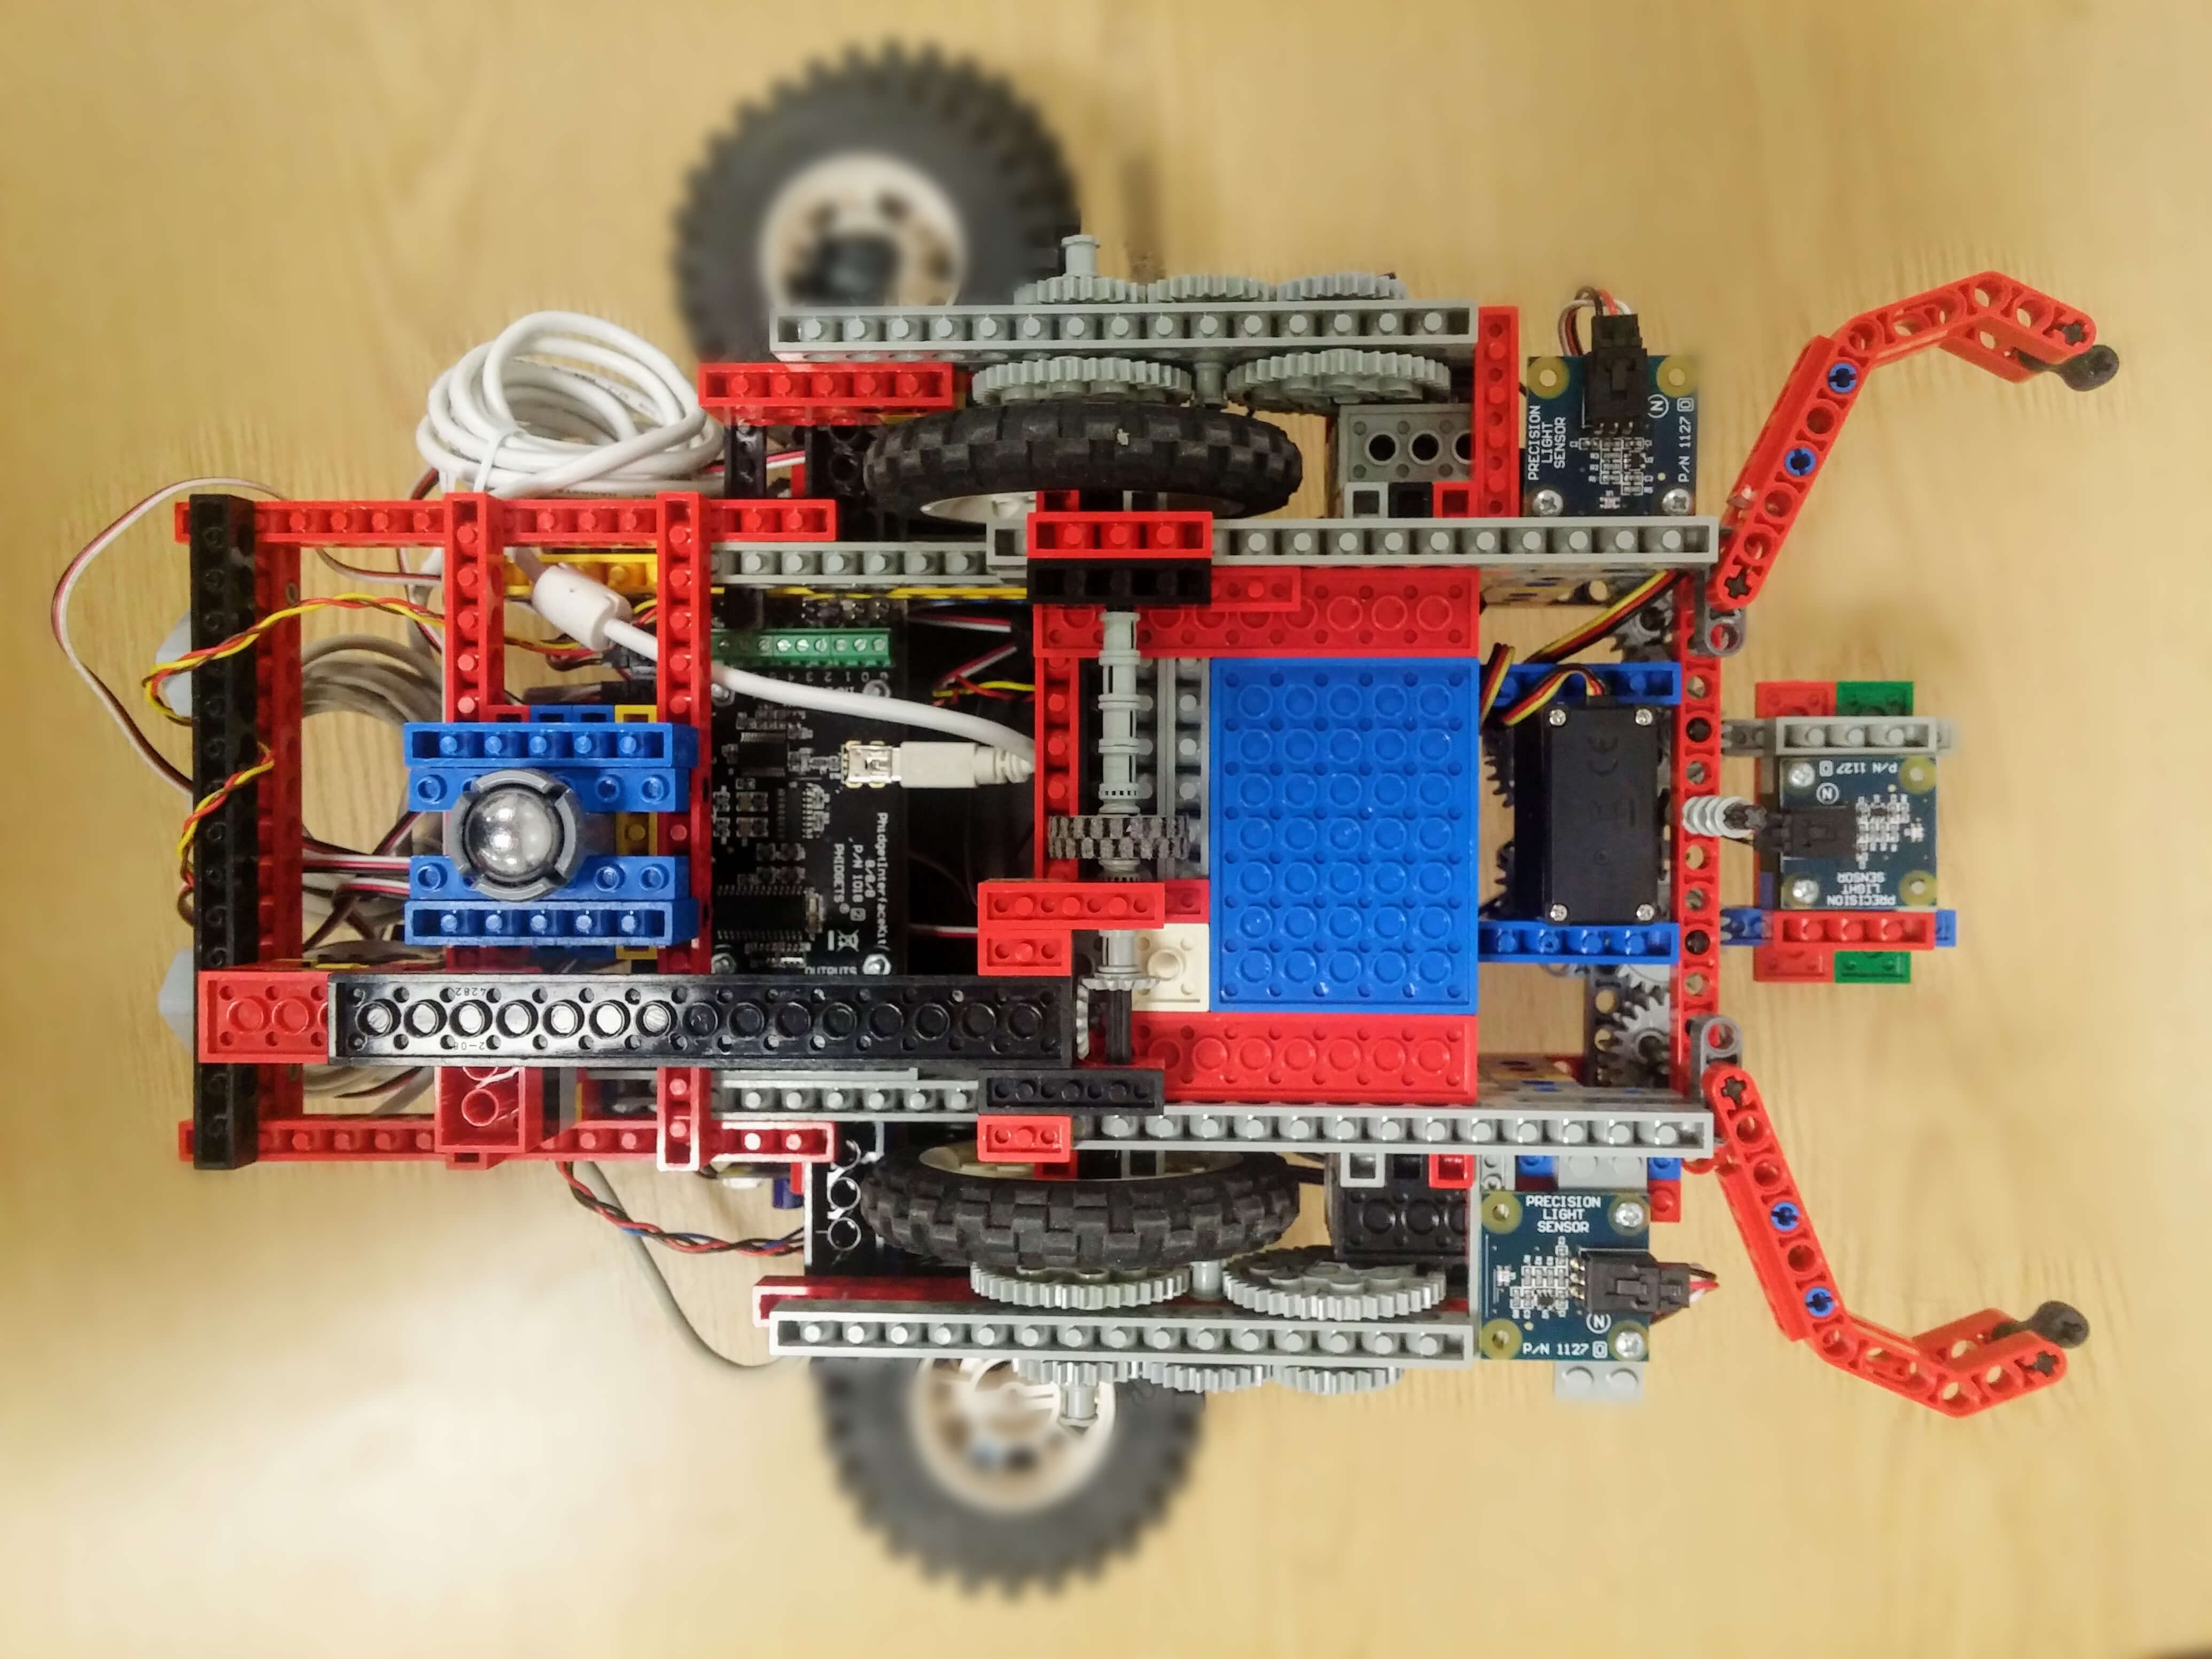
\includegraphics[height=0.8\linewidth, angle=90]{res/robot-pics/view-bottom.jpg}
    \caption{
        Bottom view of the robot. The caster wheel can be seen on the left of the image, and the two large rubber wheels on the center. The other wheels on the blurry background are not part of the robot and were used just to support the upside down robot while this shot was taken.
    }
\end{figure}

To take advantage of the quite heavy battery of the robot, it was placed as close to the front wheels as possible. Doing this added pressure on the tyres of the wheels, increasing the friction between them and the ground of the arena - which is considerably slippy from all the dust.

The power boards and the Fit PC were mounted on the back of the robot, between the two front wheels and the caster wheel. Doing this, and placing the battery close to the front wheels ensured that the center of mass would stay between all the wheels, approximately evenly distributed by them. This was a crucial element of the robot's design.

\begin{figure}[ht]
    \centering
    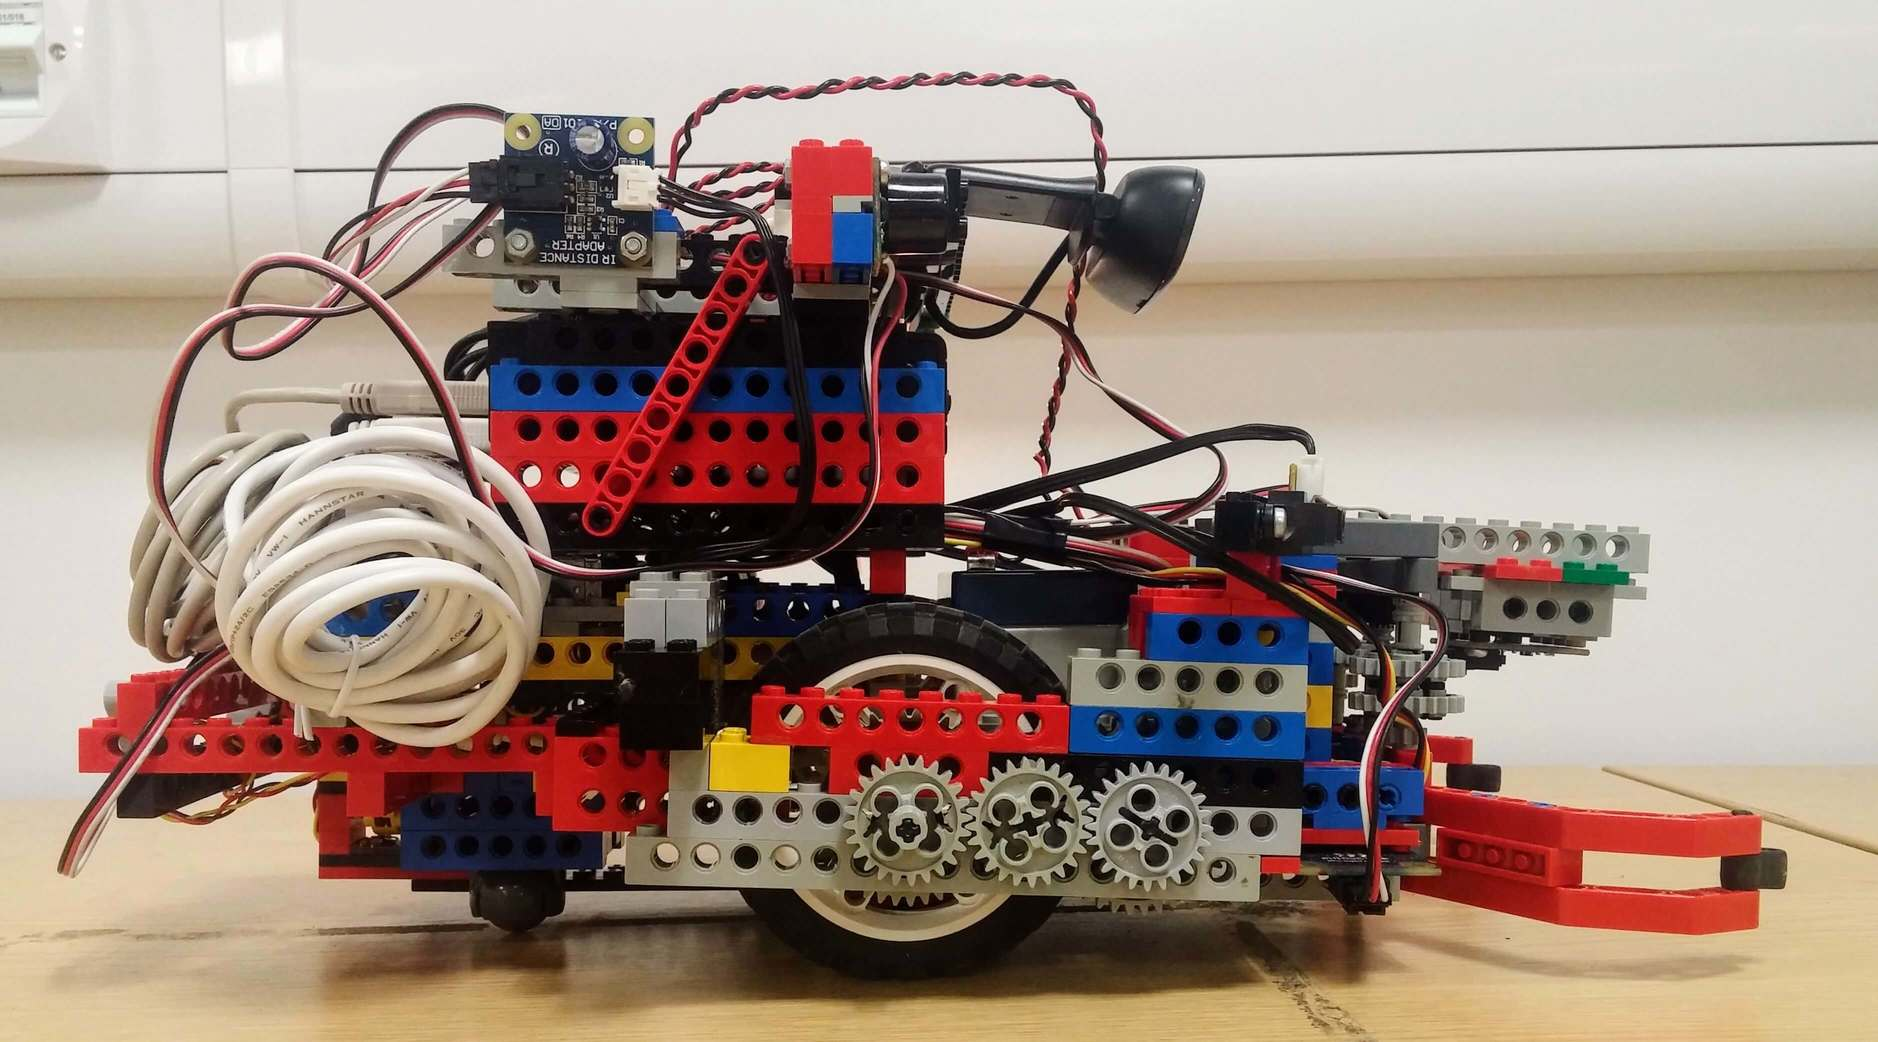
\includegraphics[width=0.8\linewidth]{res/robot-pics/view-right-side.jpg}
    \caption{View of the right side of the robot.}
\end{figure}

\clearpage

It was decided from the very start that the main Power Board should be easily accessible to plug the AC adaptor and to turn On/Off the DC motor power board. For that reason, the Power Board was placed on the very top of the robot, just behind the camera.

The need to constantly plug and unplug sensors to the Phidgets Boards made it clear that there should be an easy way to get to those sensor slots. This was even more important with the constant battery switching when they ran out of power. To solve this problem, a \textit{Hop On - Hop Off} with hinges was devised. To gain access to the boards and to the battery slot, one needed only to lift the hop.

\begin{figure}[ht]
    \centering
    \begin{subfigure}{0.49\textwidth}
        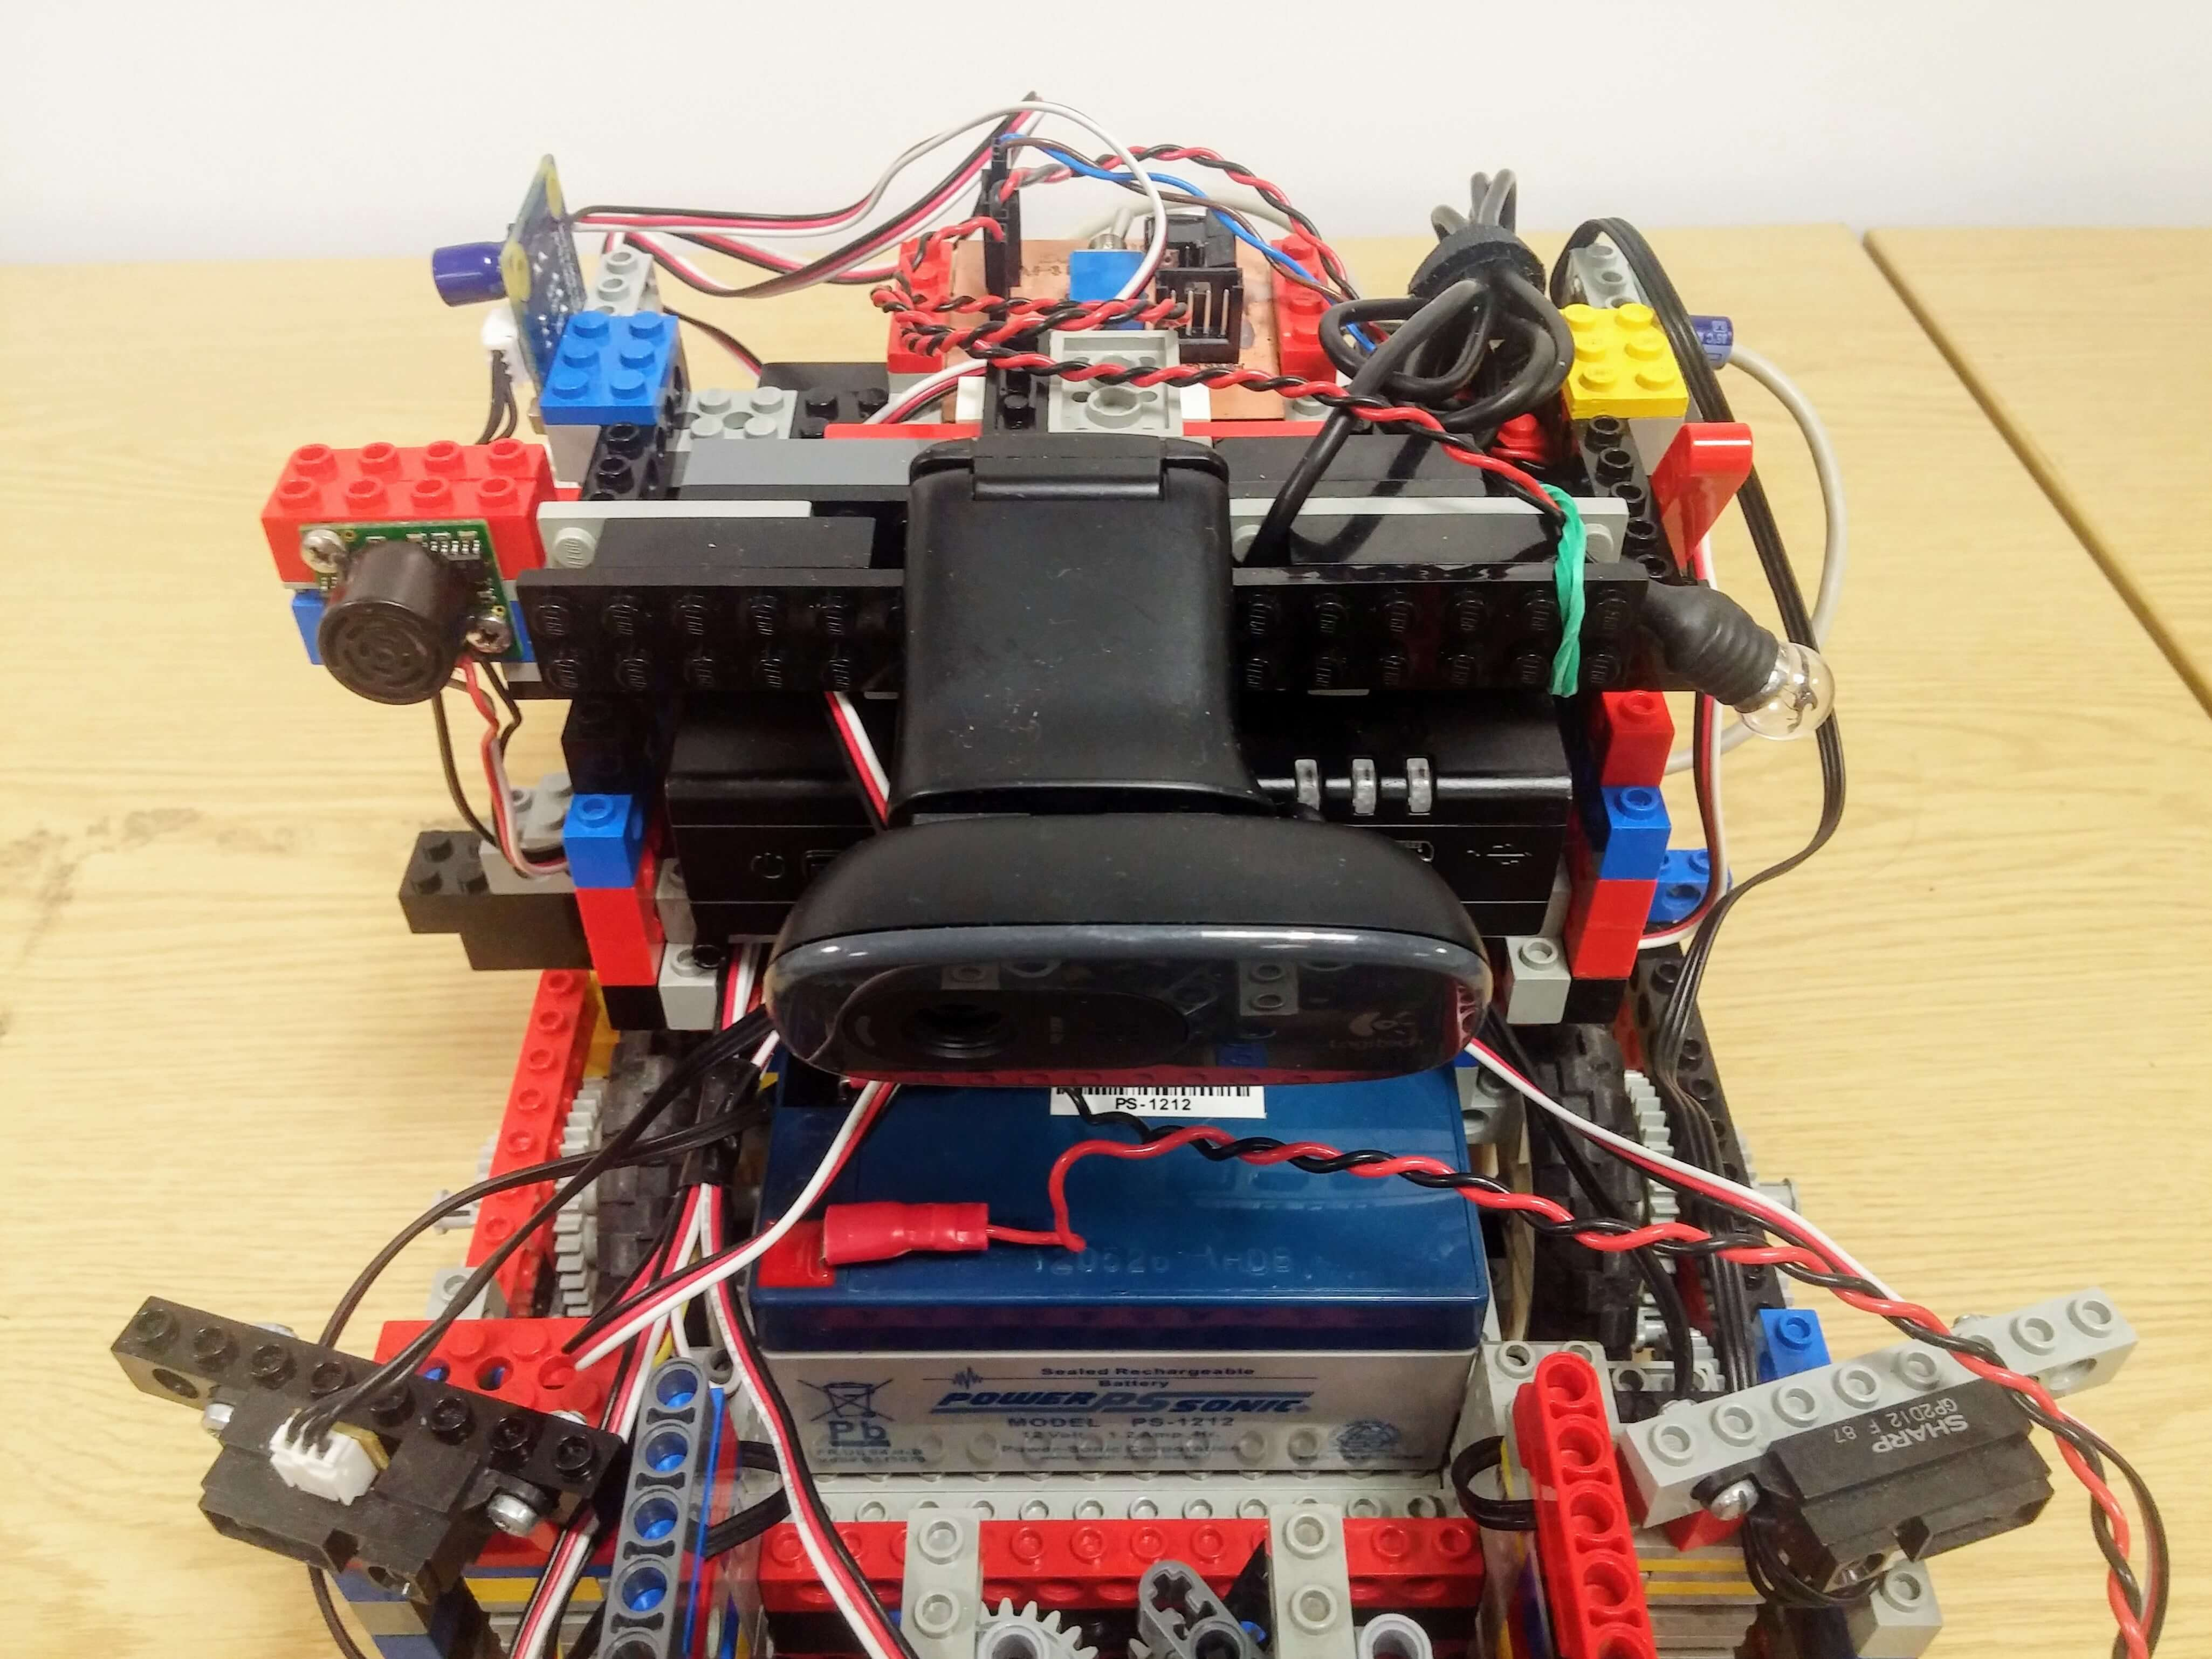
\includegraphics[width=\linewidth, height=4cm]{res/robot-pics/top-on.jpg}
        \caption{Hop on}
        \label{fig:hop-on}
    \end{subfigure}
    \begin{subfigure}{0.49\textwidth}
        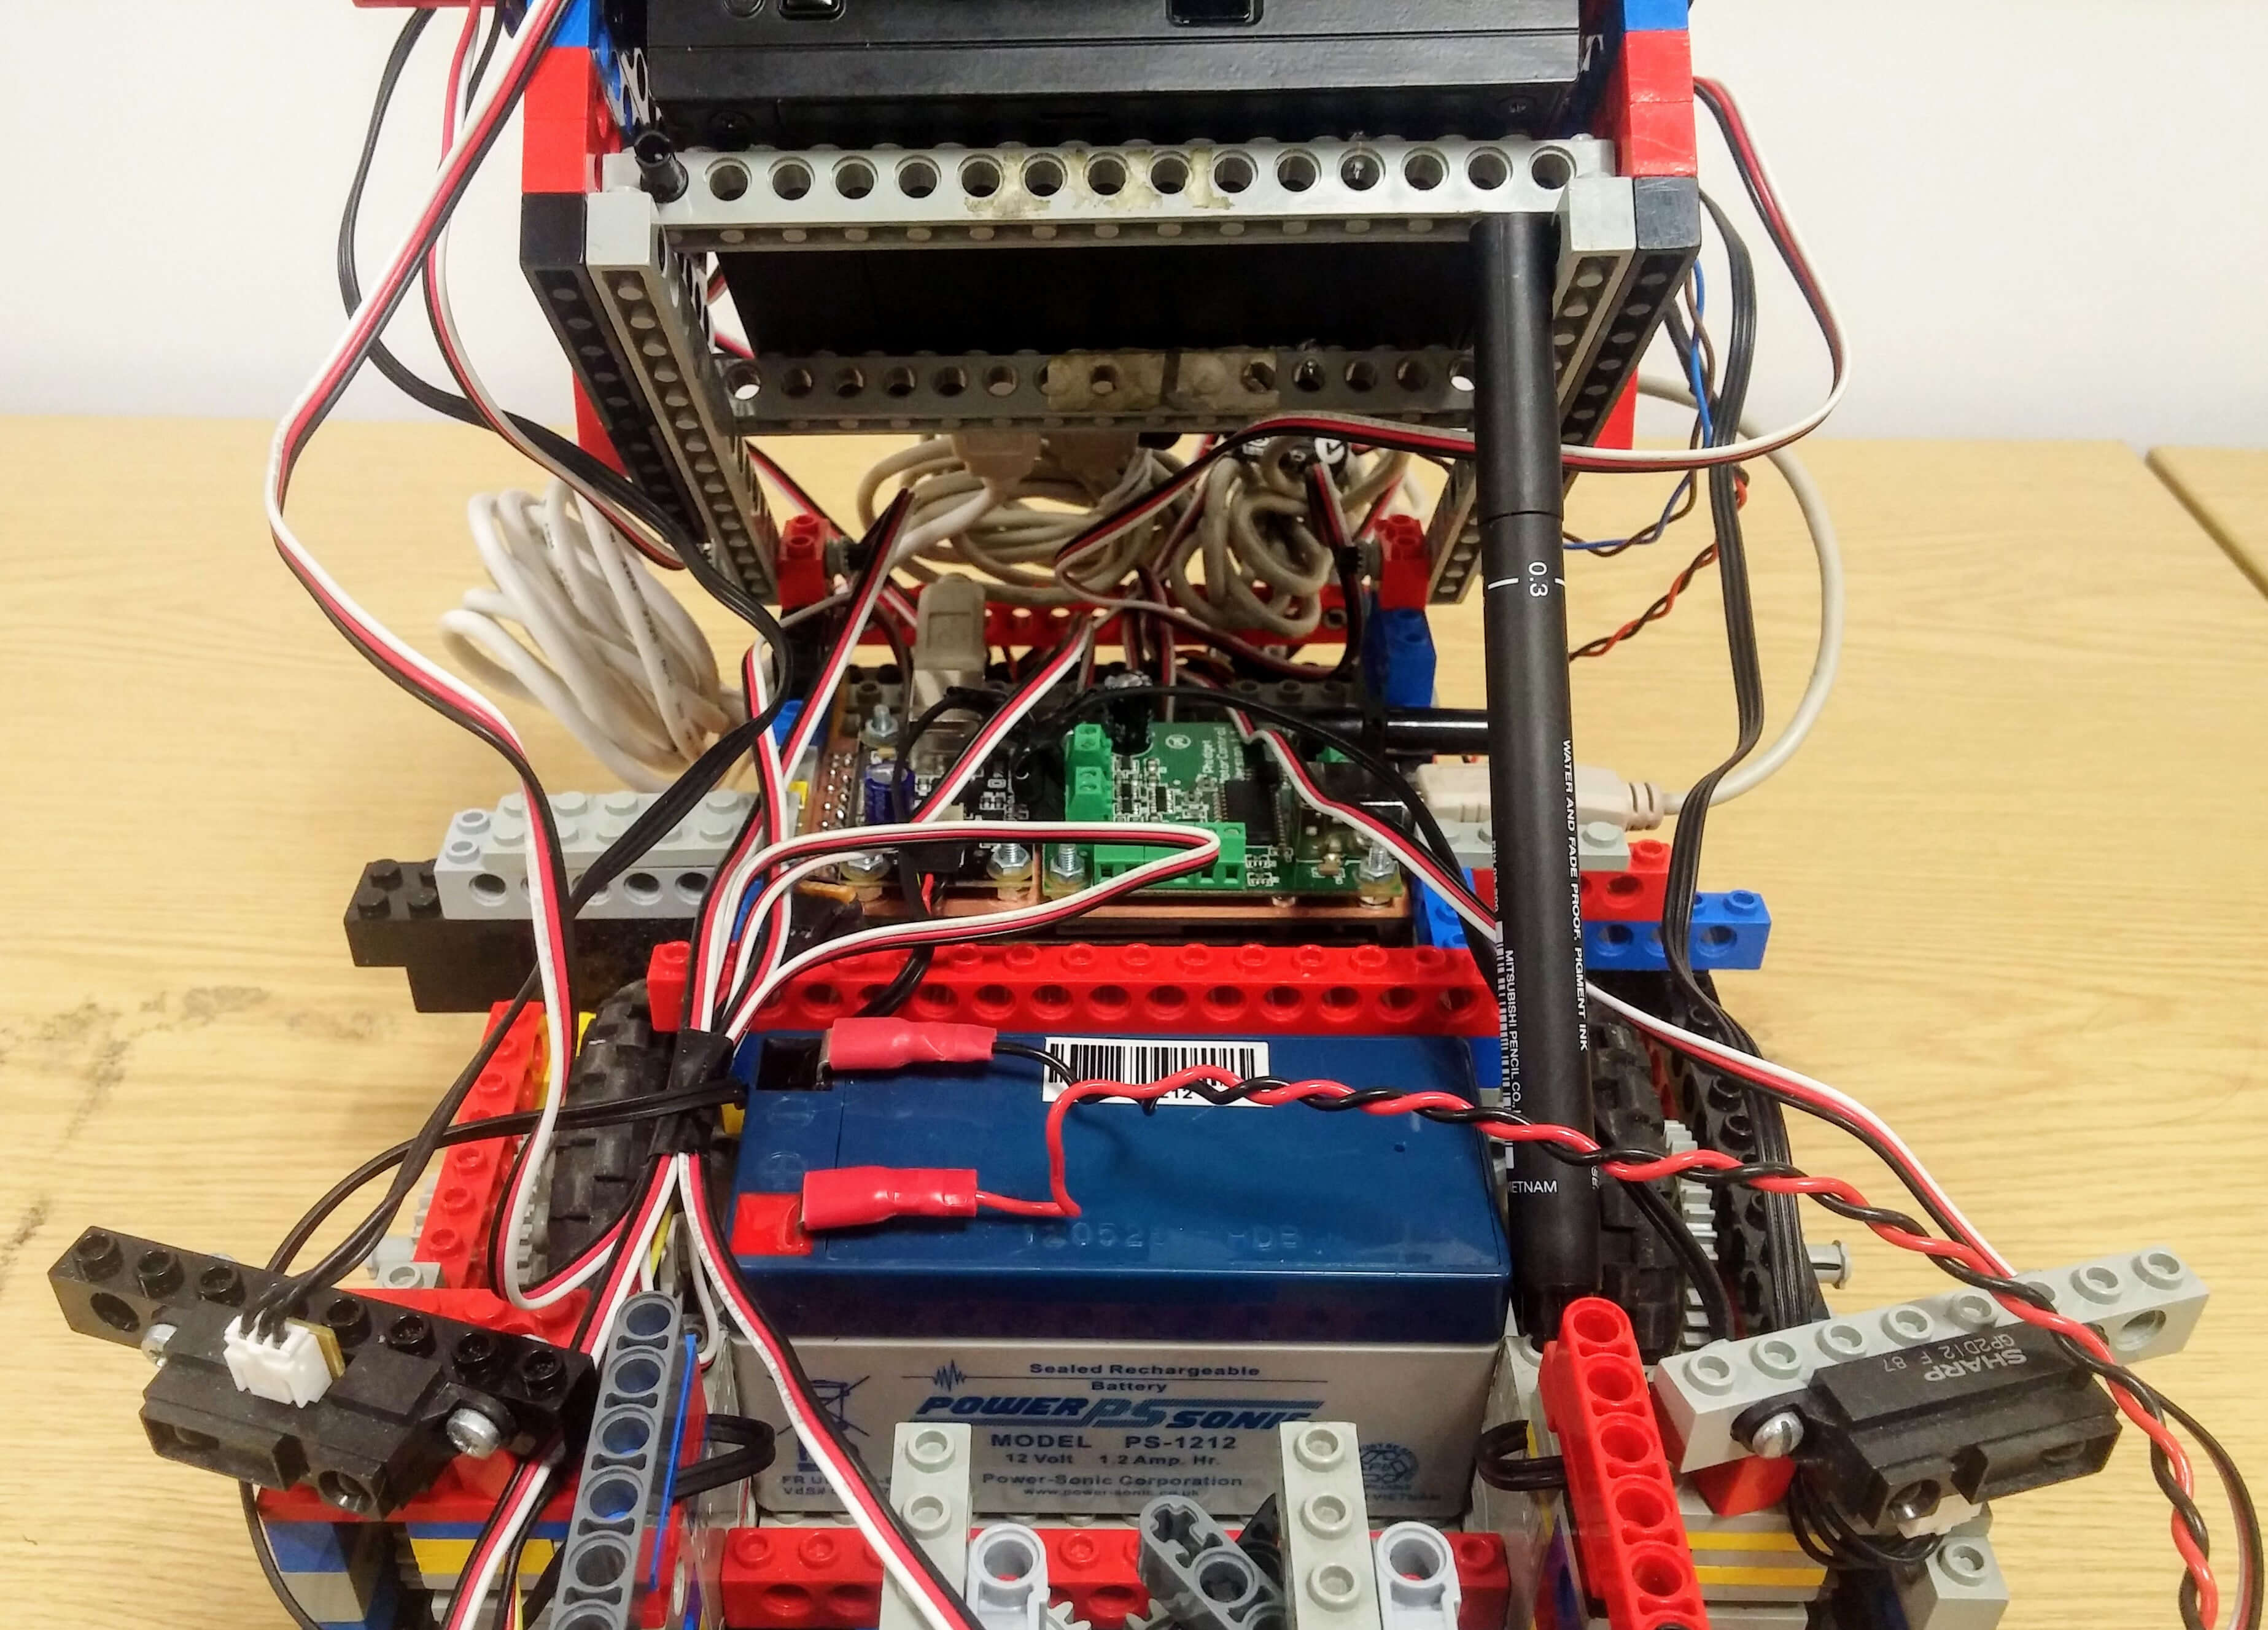
\includegraphics[width=\linewidth, height=4cm]{res/robot-pics/top-off.jpg}
        \caption{Hop off}
        \label{fig:hop-off}
    \end{subfigure}
    \caption{Lifting the hop reveals the Phidgets boards and enables easy access to the battery slot.}
    \label{fig:hop-on-off}
\end{figure}

% - - - - - - - - - - - - - - - - - - - - - - - - - - -

\subsection{Base detector and gripper}

The gripper had to be placed on the front in order to catch the cubes when the robot drove to them. The precision servo motor was used to open or close the gripper handles.

One light sensor was mounted facing down on top of the gripper dock, at such a height that a cube would fit just underneath it. Since the cubes are textured on the sides, but are solid black on the top and bottom, placing the light sensor in such position made it very easy for the robot to detect whenever there was a cube on its gripper dock or not.

To complement the gripper, two more light sensors were placed at the front of the robot, one in each side, just hovering the floor and facing down.\\
These constituted the base detector for the black rectangular bases on the arena, and they functioned very similarly to the cube detector on the gripper: they measured the amount of light reflected by the gray floor of the arena, and triggered whenever black was being sensed instead of gray - this meant that that sensor was on one of the bases.\\
When the robot moved forward, carrying a cube and suddenly both light sensors from the base detector got triggered, it meant the robot had arrived to the base and it could release the cube to deliver it.

\begin{figure}[ht]
    \centering
    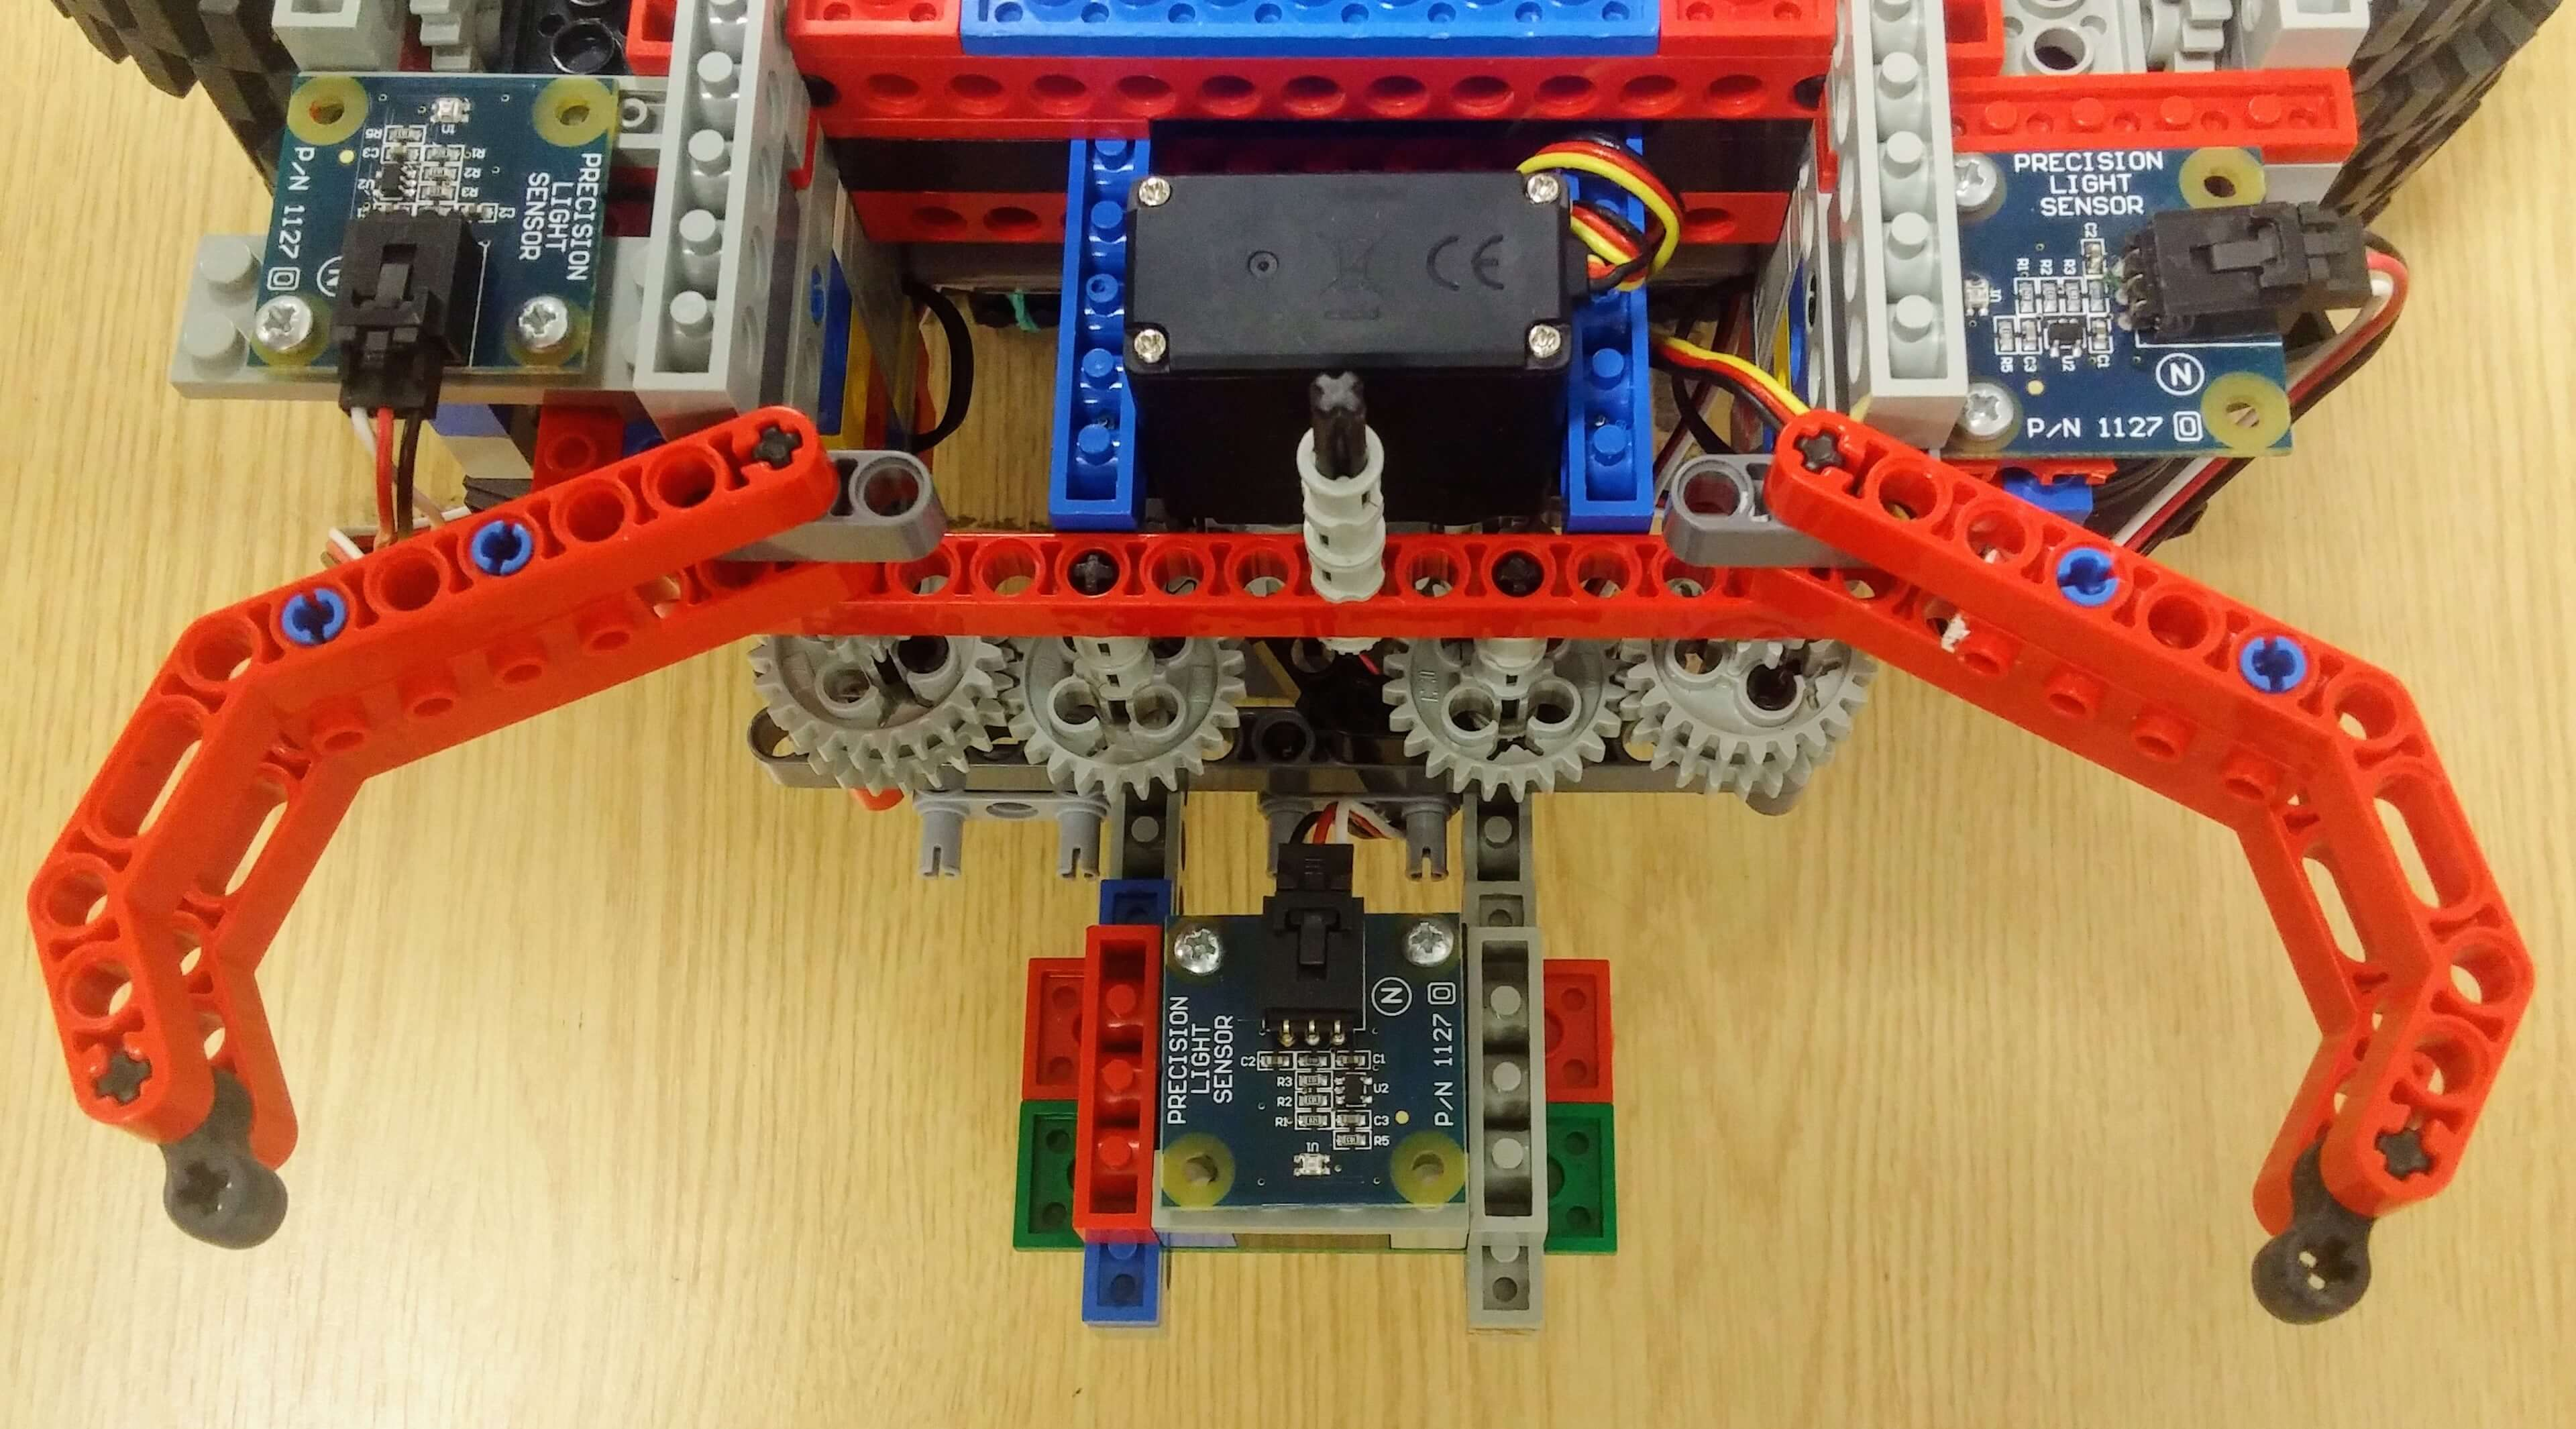
\includegraphics[width=0.7\linewidth]{res/robot-pics/base-detector-and-gripper.jpg}
    \caption{The base detector light sensors can be seen on the left and right top corners of this image. On the center, there is the precision servo motor, the gear train to open or close the gripper, and finally, on the middle bottom, the cube detection light sensor.}
    \label{fig:base-detector-and-gripper}
\end{figure}

% - - - - - - - - - - - - - - - - - - - - - - - - - - -

\subsection{Actuators and gearing}

\begin{figure}[ht]
    \centering
    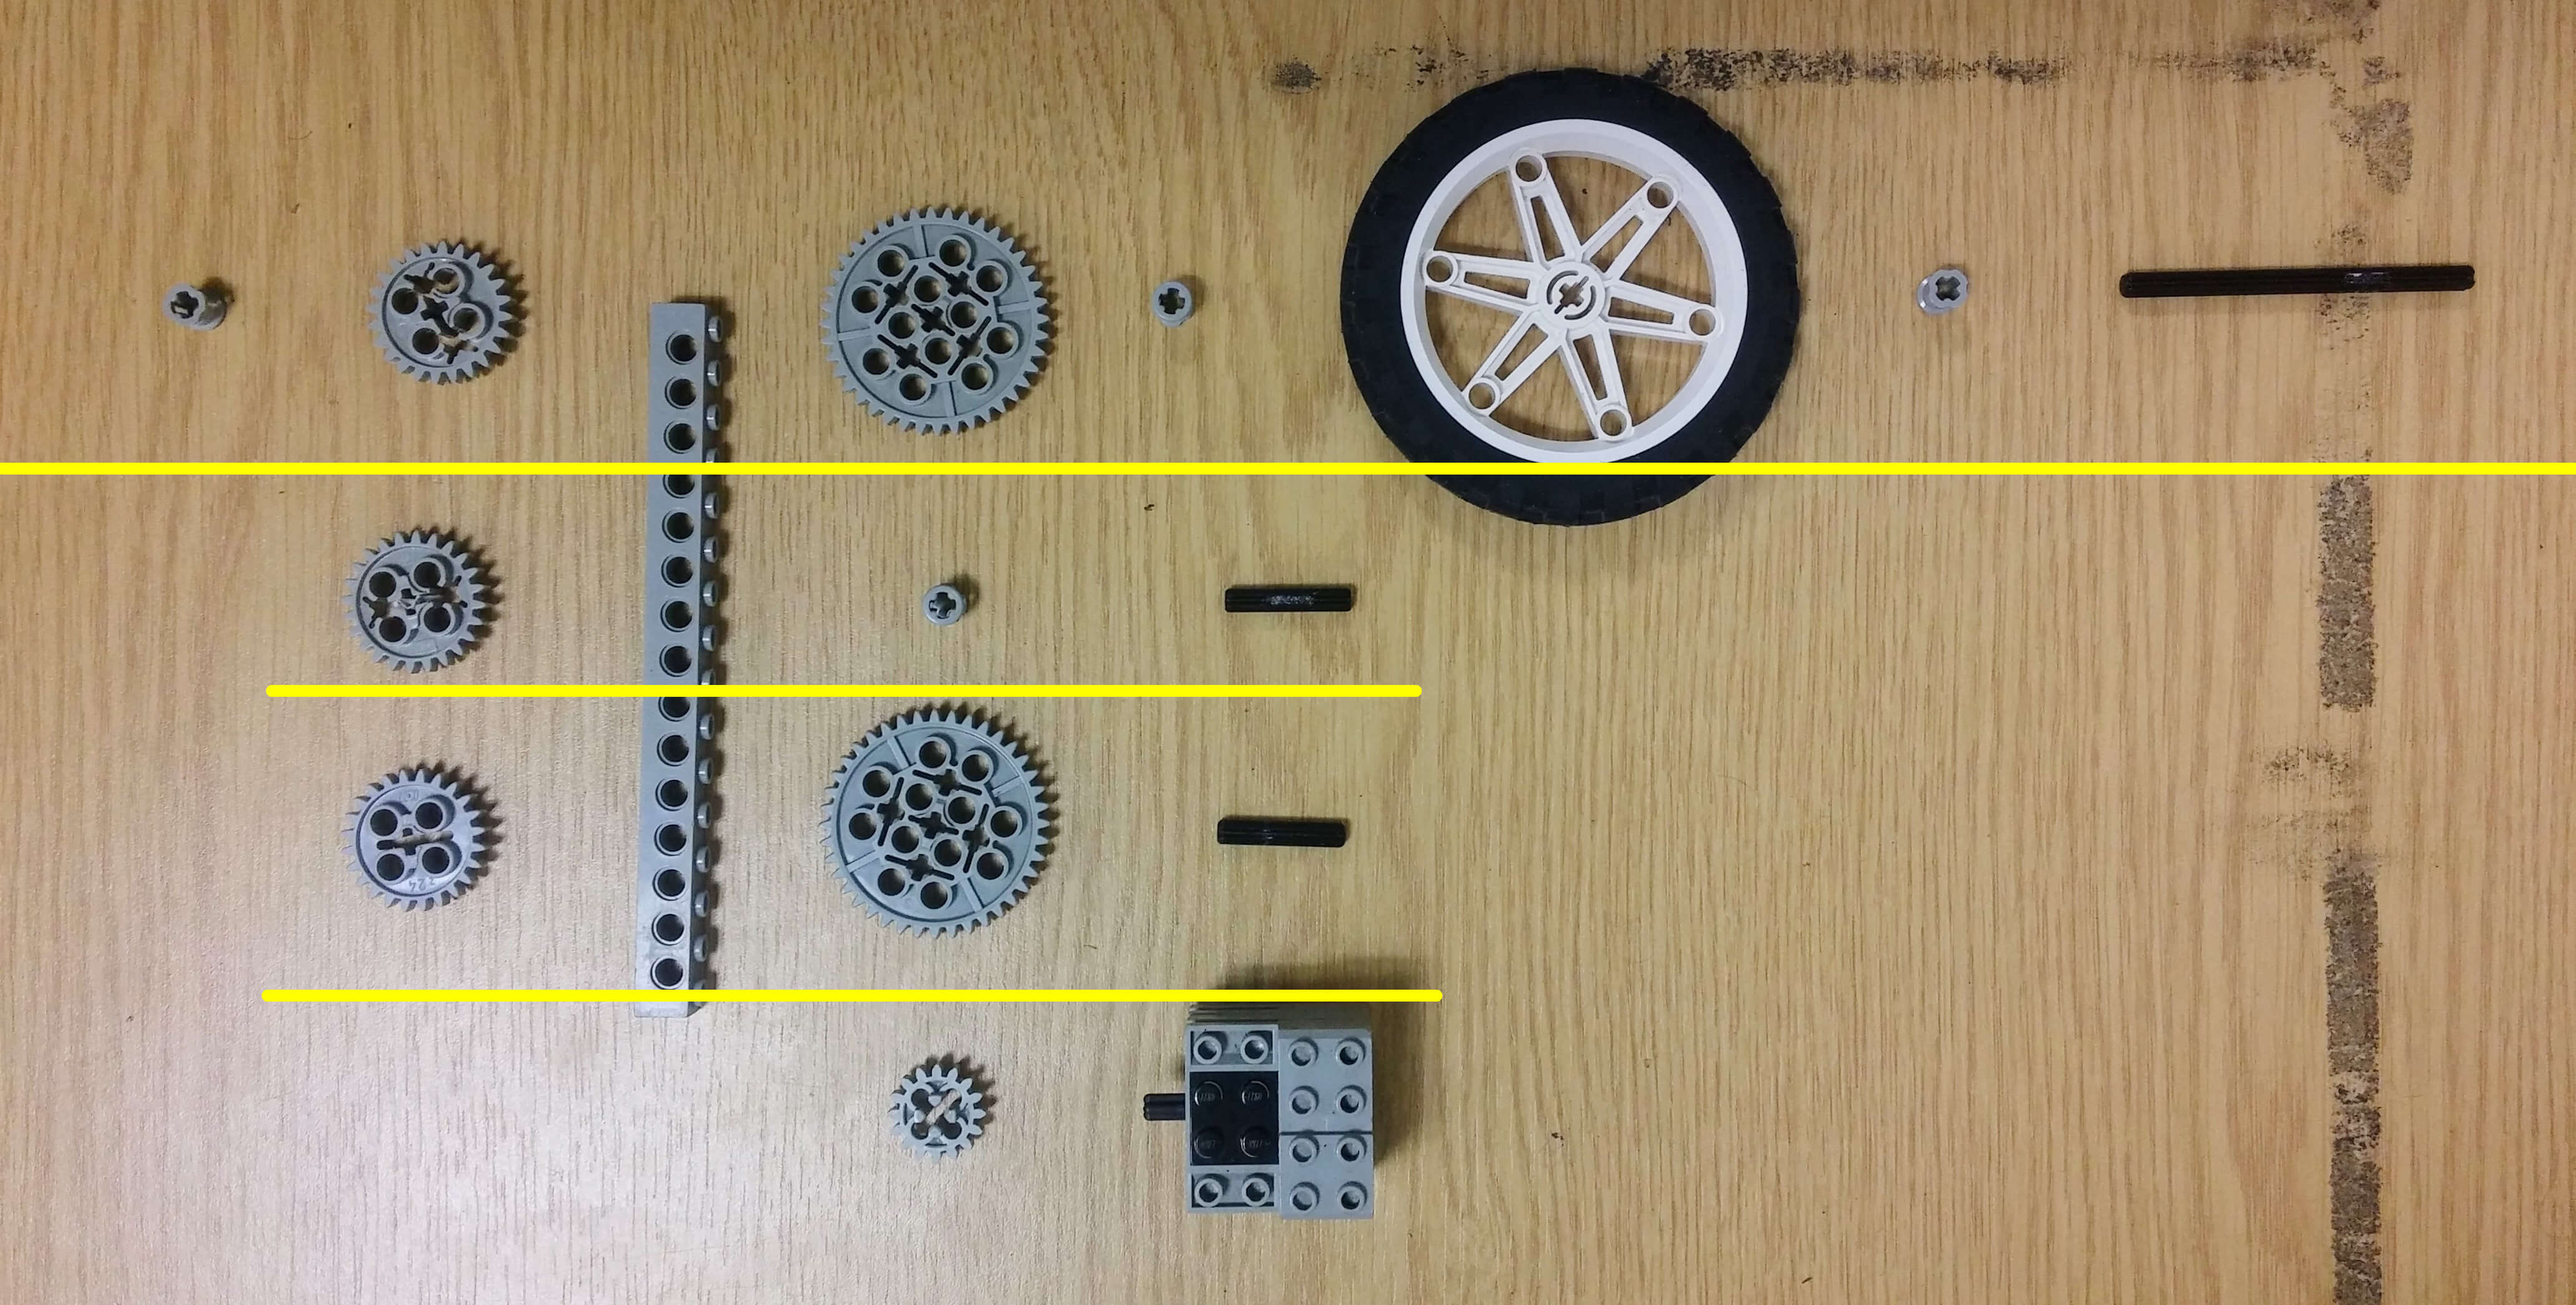
\includegraphics[width=0.7\linewidth]{res/robot-pics/gear-train-unmounted.jpg}
    \caption{}
    \label{fig:}
\end{figure}

\begin{figure}[ht]
    \centering
    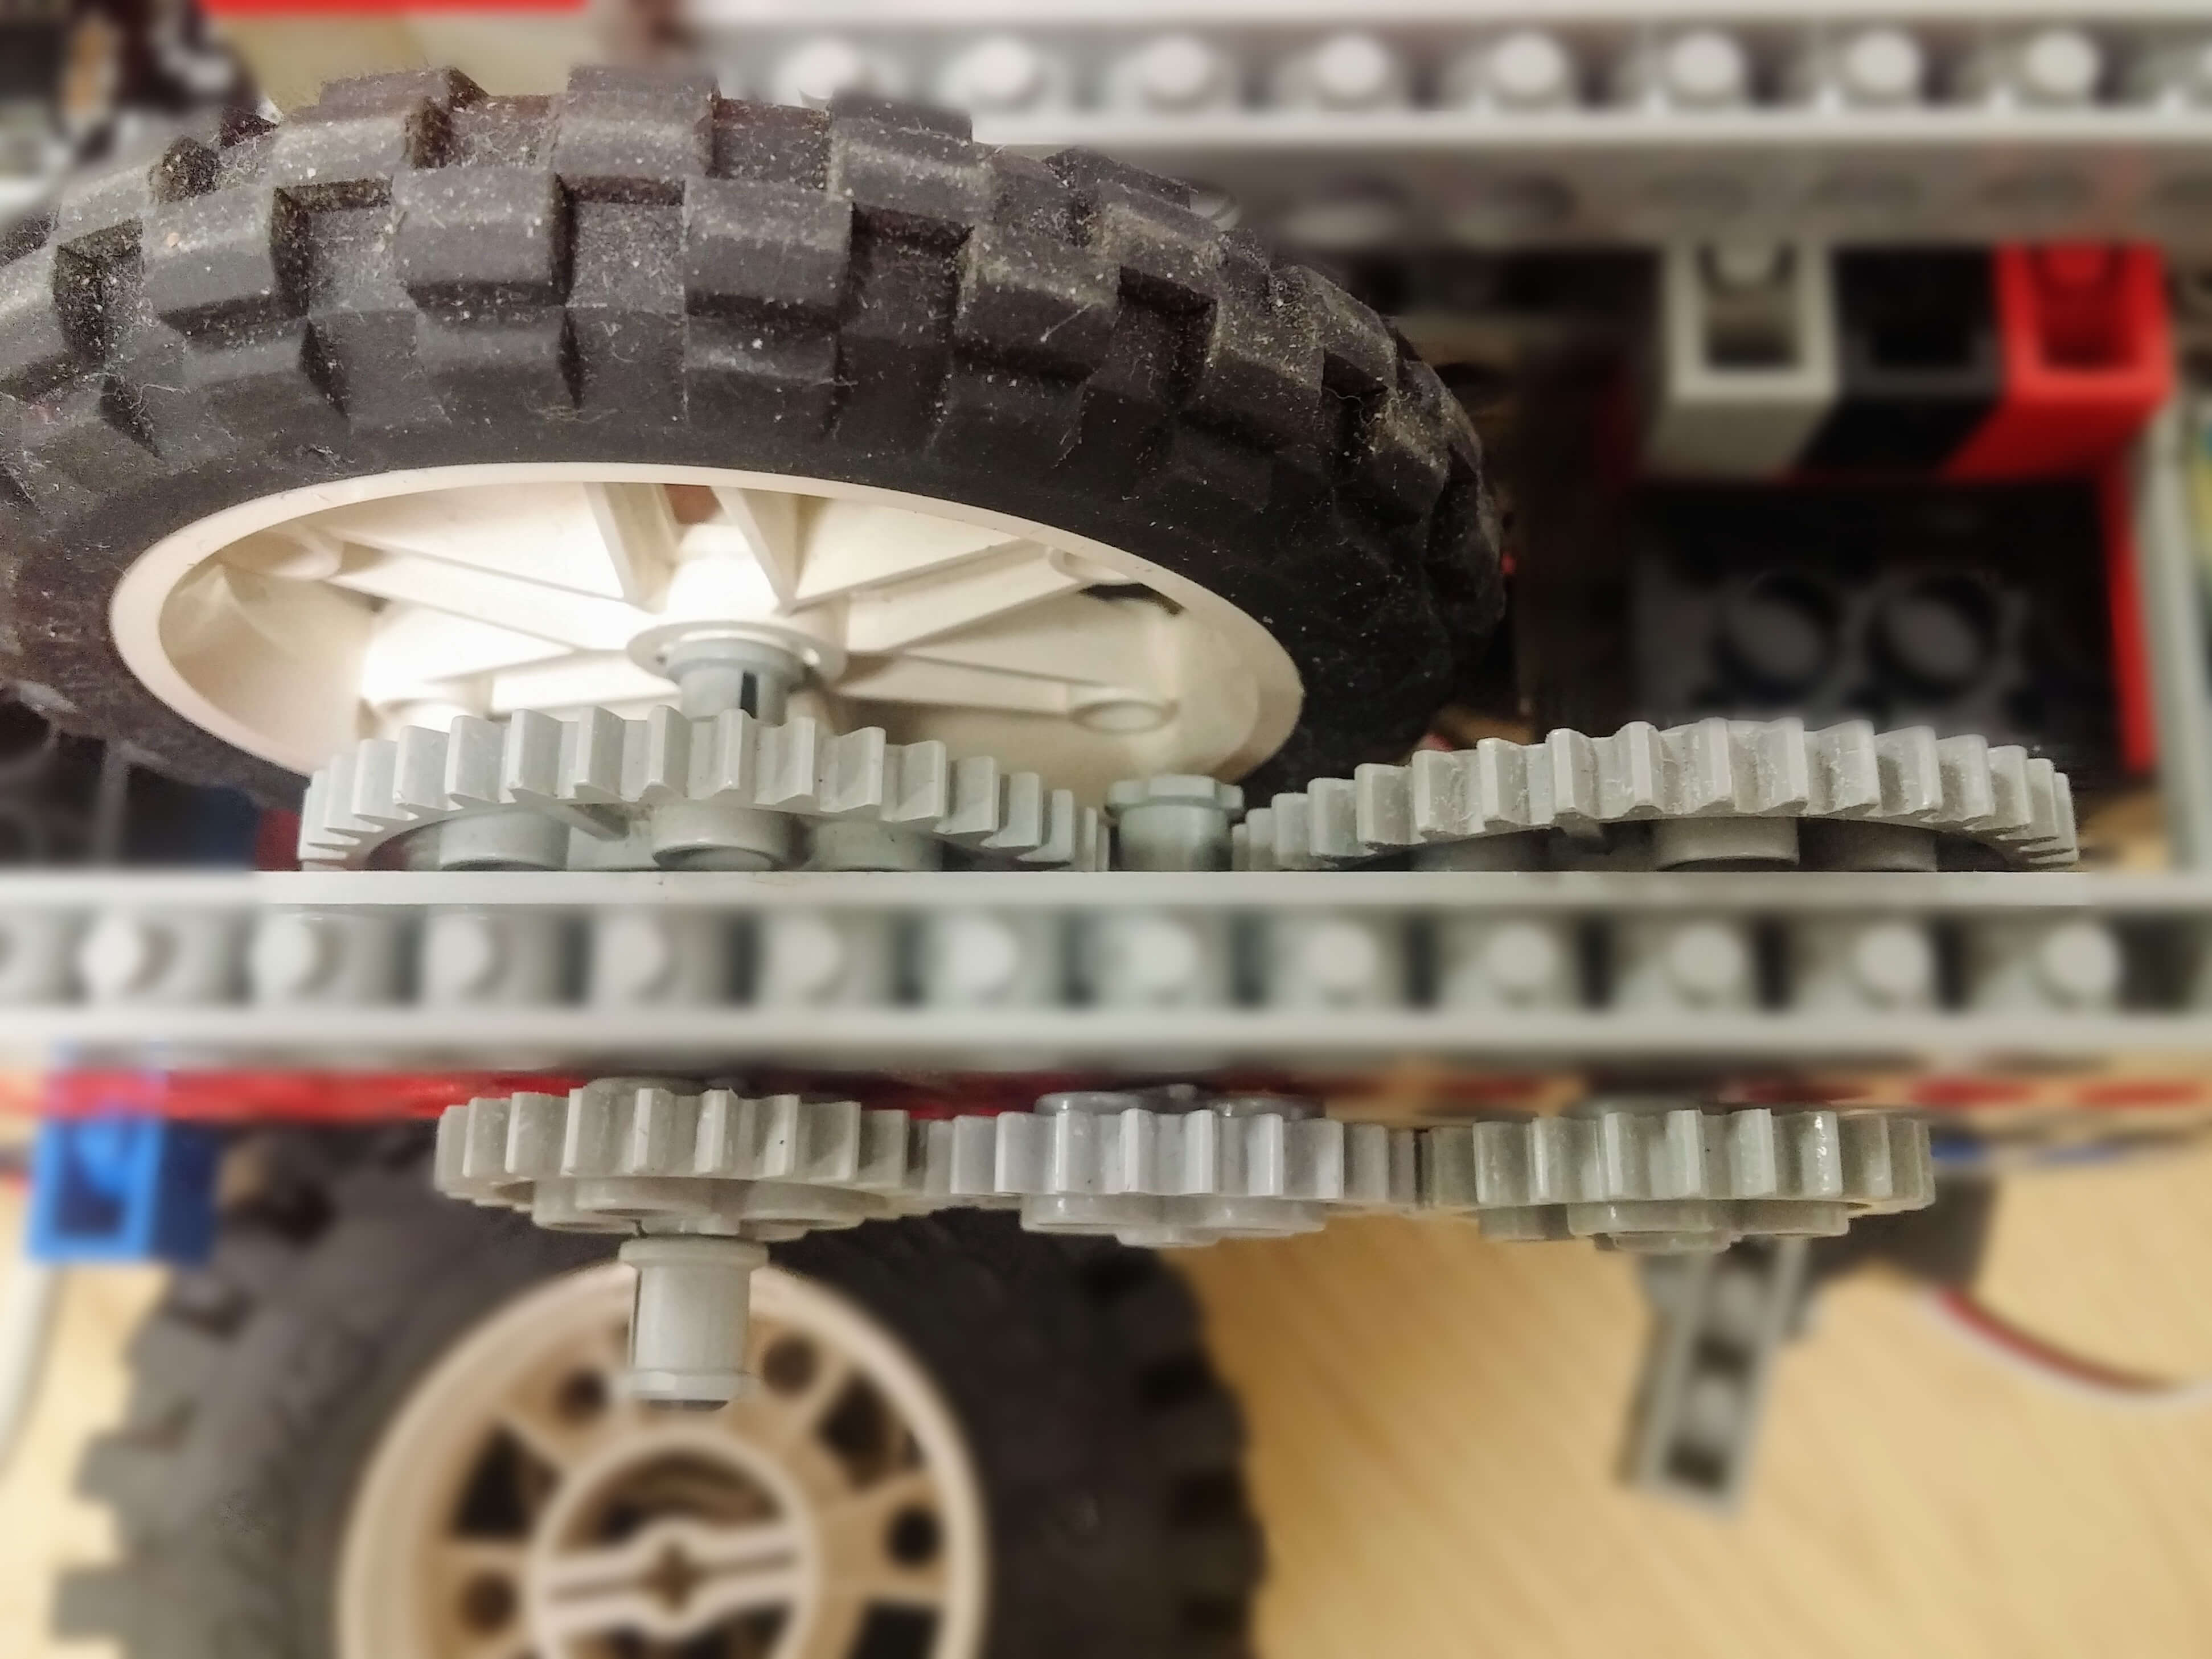
\includegraphics[width=0.7\linewidth]{res/robot-pics/gear-train-mounted.jpg}
    \caption{}
    \label{fig:}
\end{figure}

% - - - - - - - - - - - - - - - - - - - - - - - - - - -

\subsection{Sensing}

\subsubsection{IR and Sonar}

\begin{figure}[ht]
    \centering
    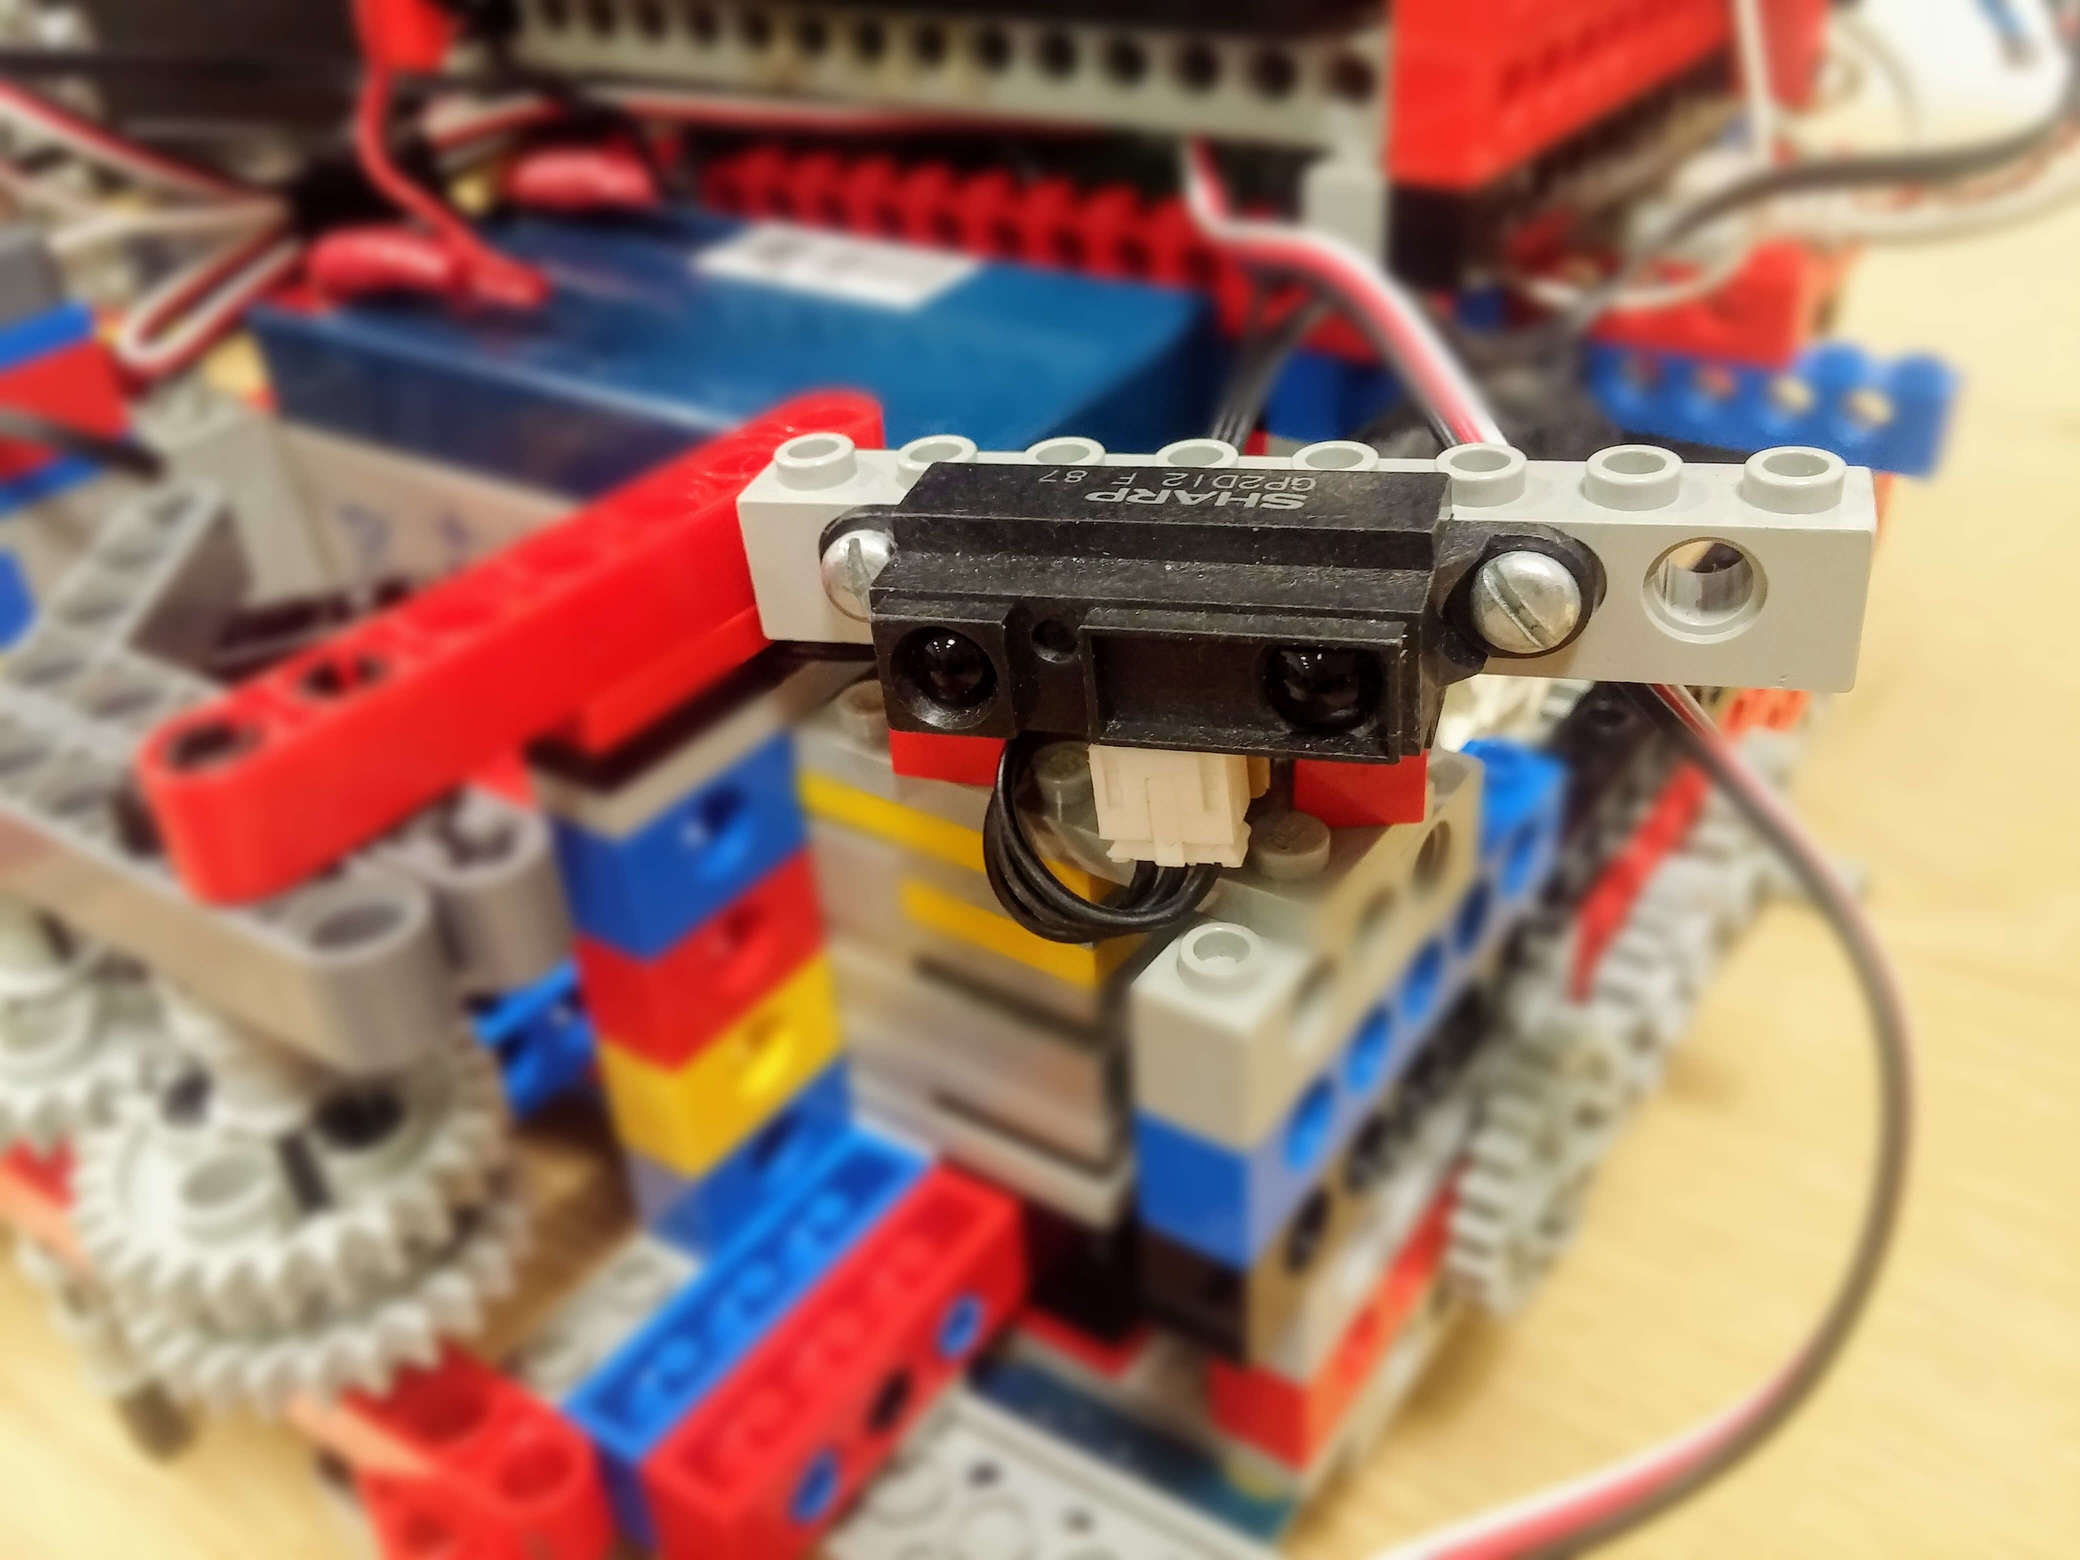
\includegraphics[width=0.7\linewidth]{res/robot-pics/ir-sensor-placement.jpg}
    \caption{}
    \label{fig:}
\end{figure}

\begin{figure}[ht]
    \centering
    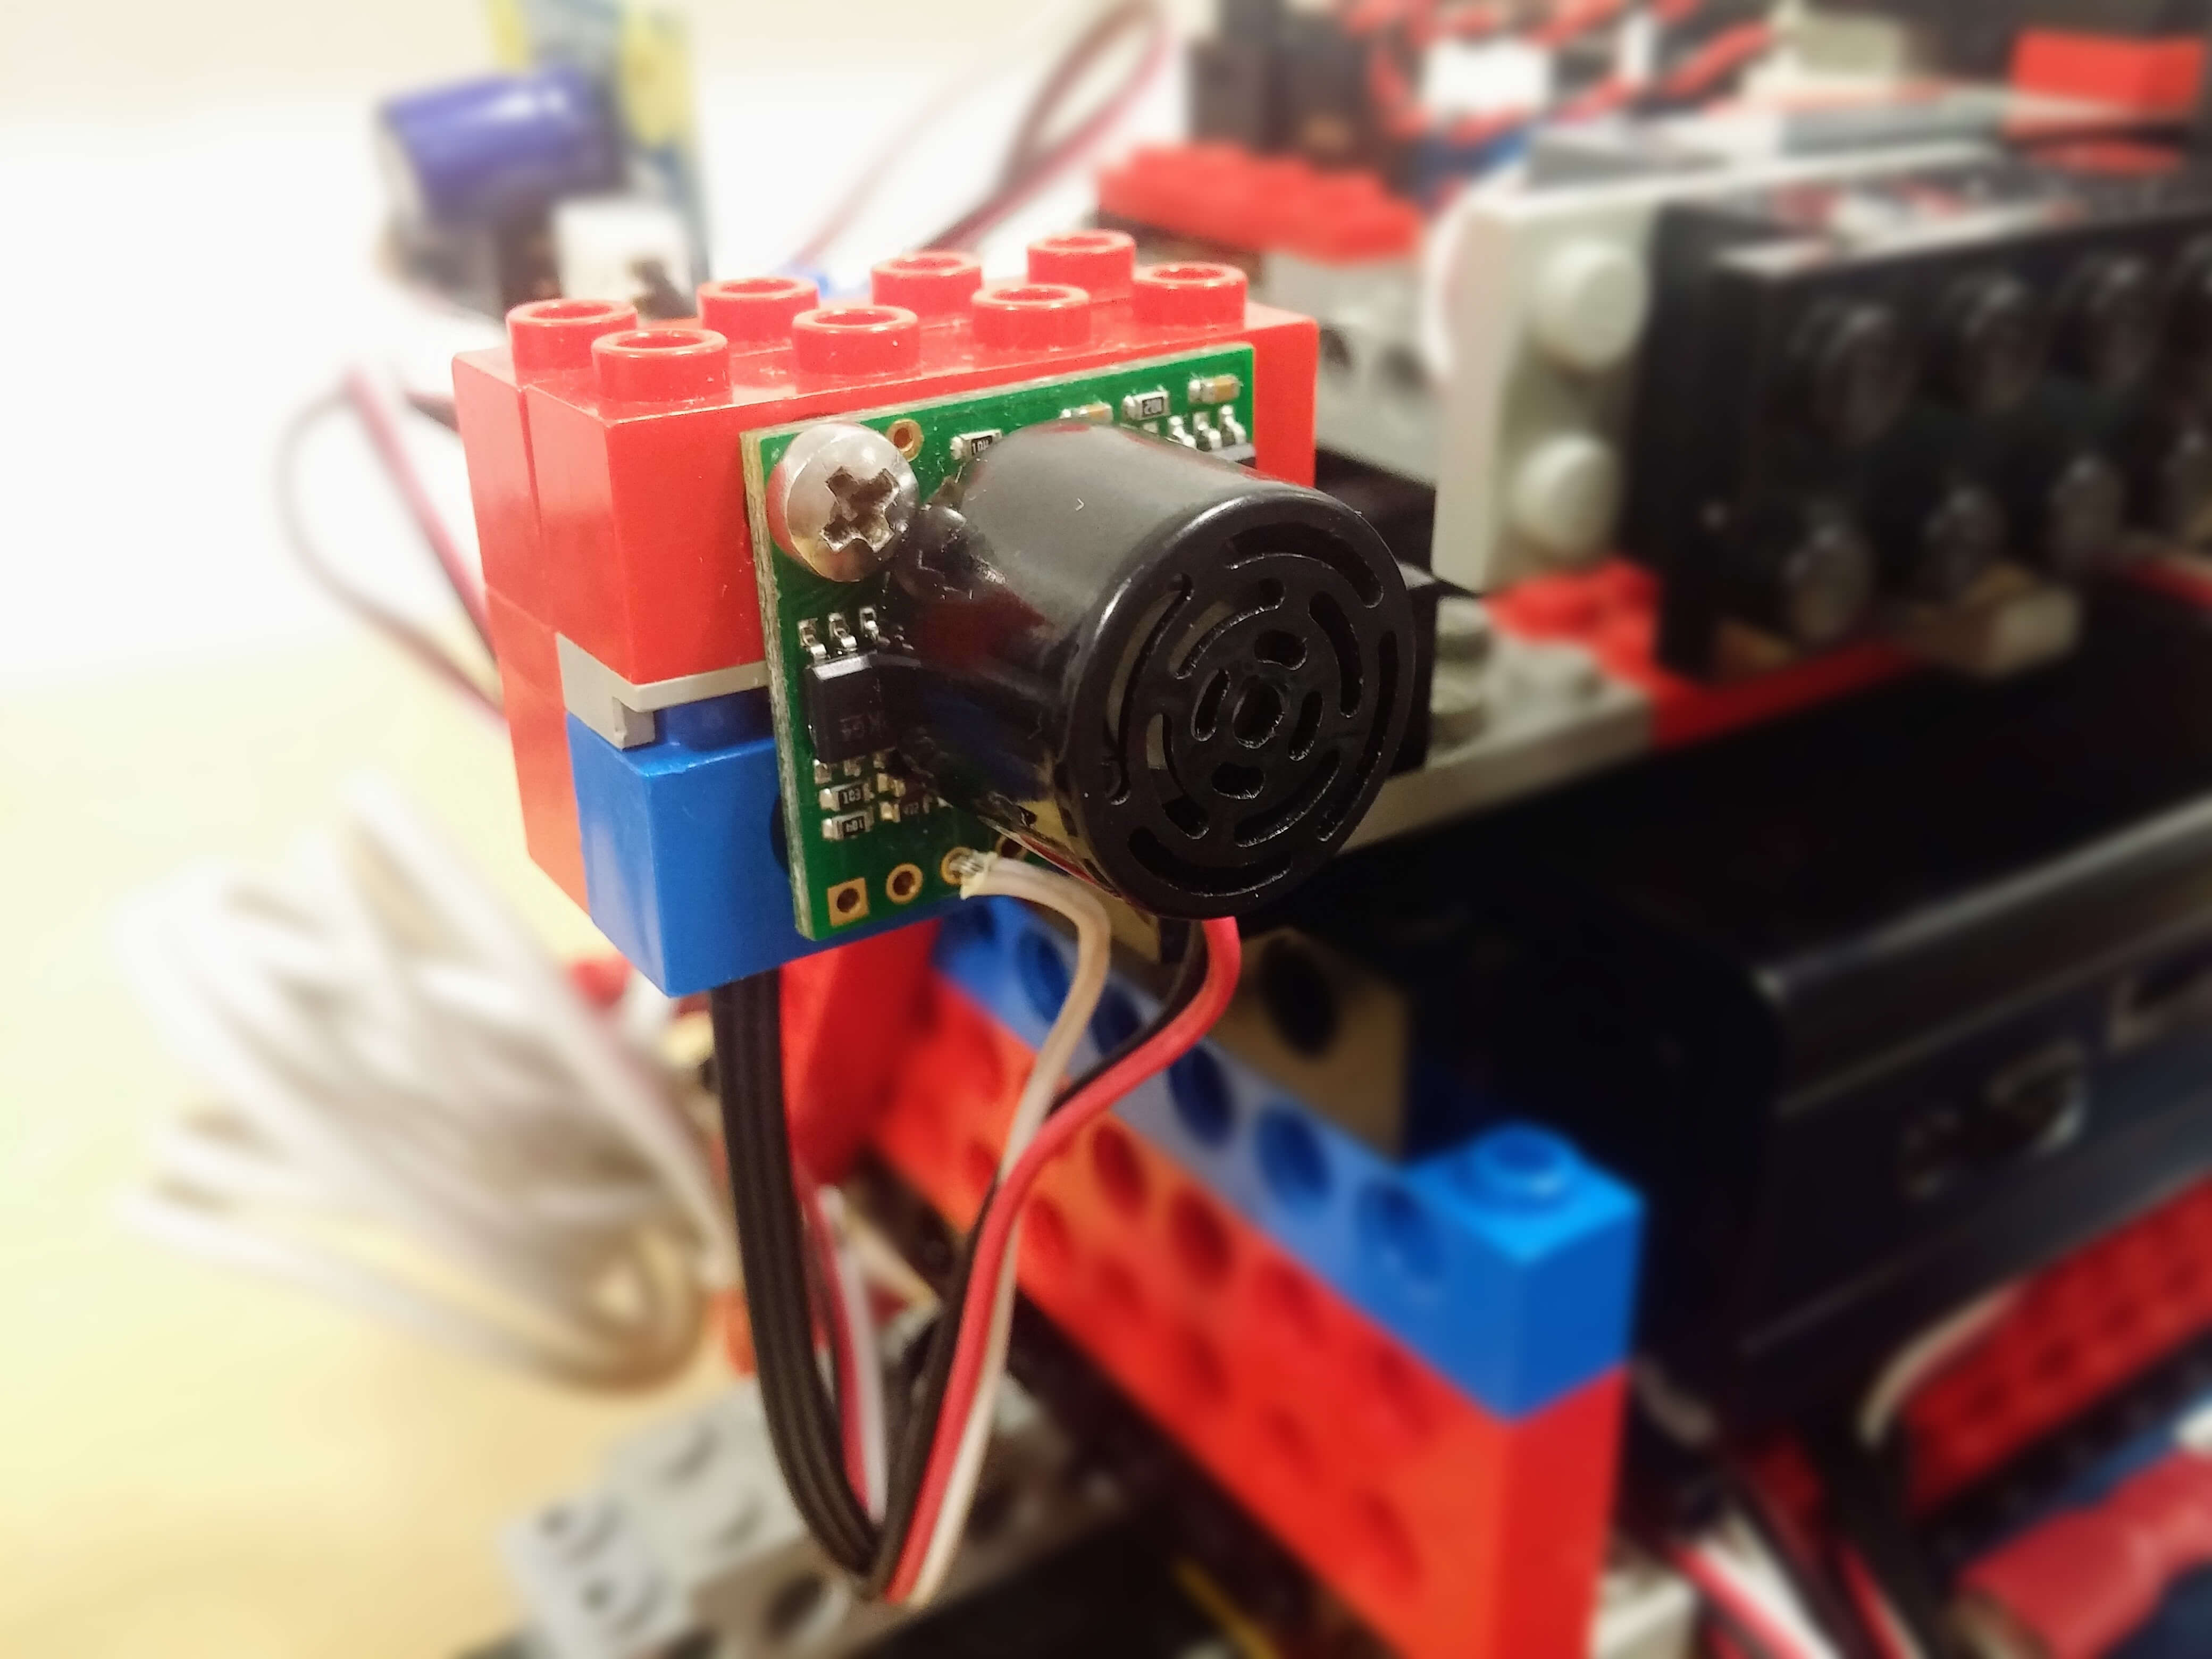
\includegraphics[width=0.7\linewidth]{res/robot-pics/sonar-placement.jpg}
    \caption{}
    \label{fig:}
\end{figure}

\subsubsection{Camera}

\begin{figure}[ht]
    \centering
    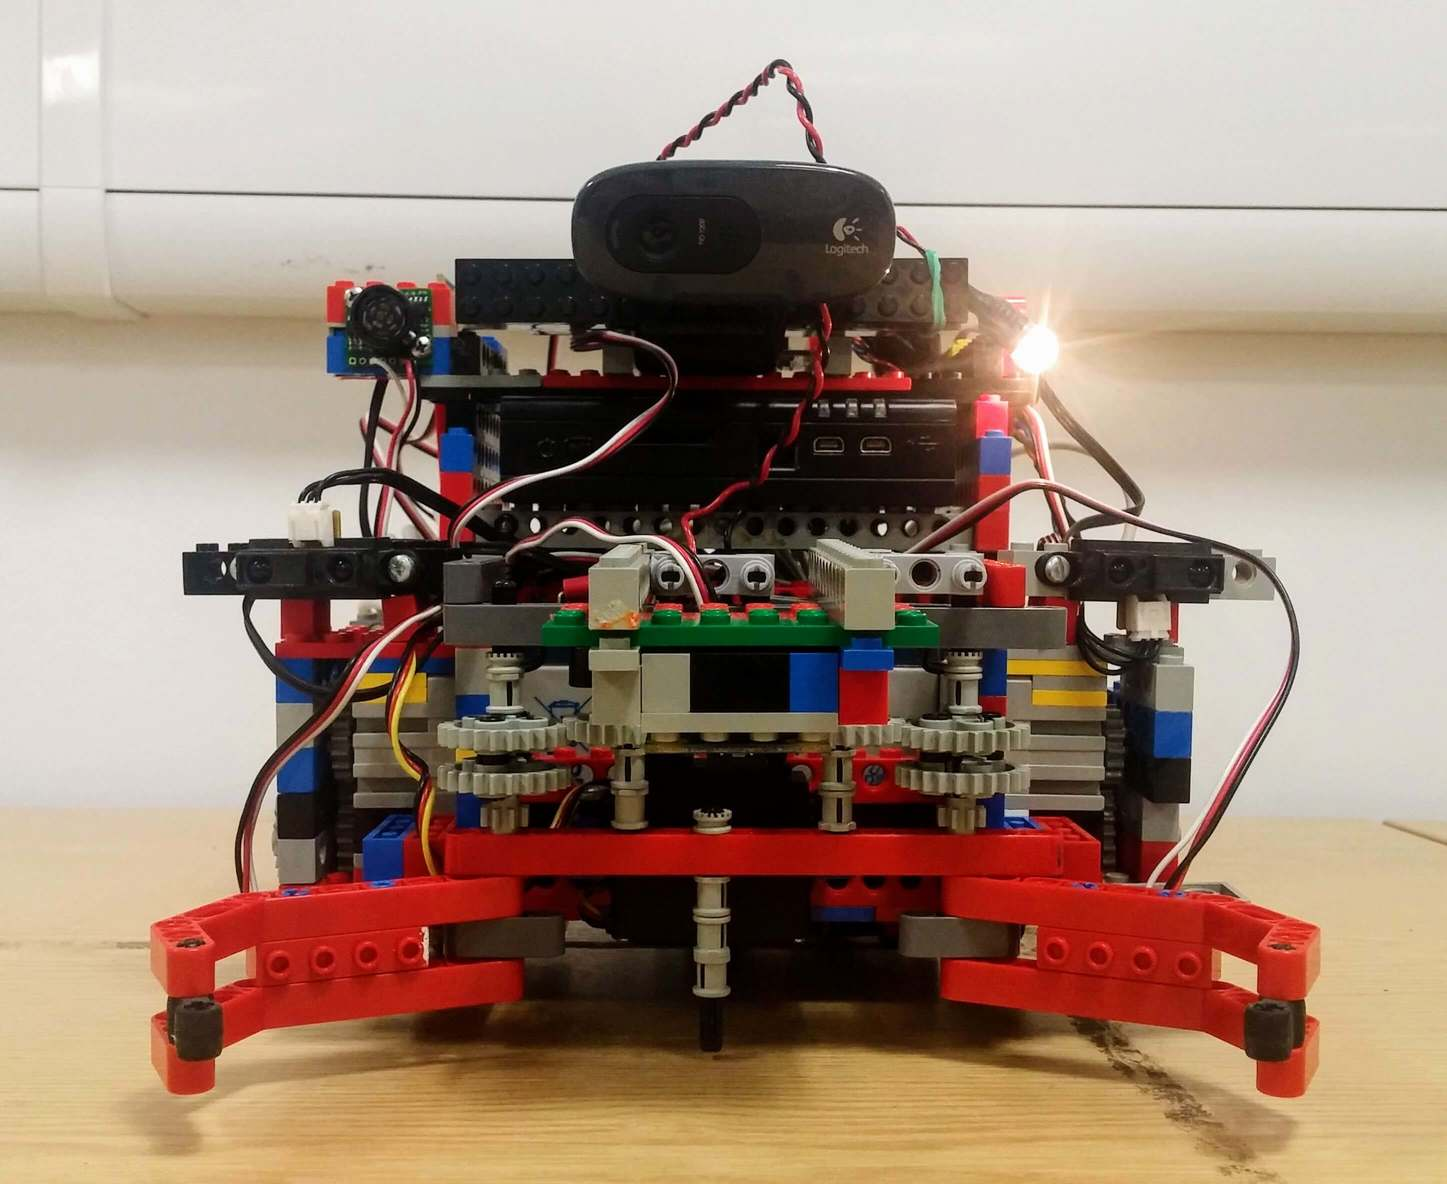
\includegraphics[width=0.7\linewidth]{res/robot-pics/view-front.jpg}
    \caption{}
    \label{fig:}
\end{figure}

\subsubsection{Hall effect sensor}

\begin{figure}[ht]
    \centering
    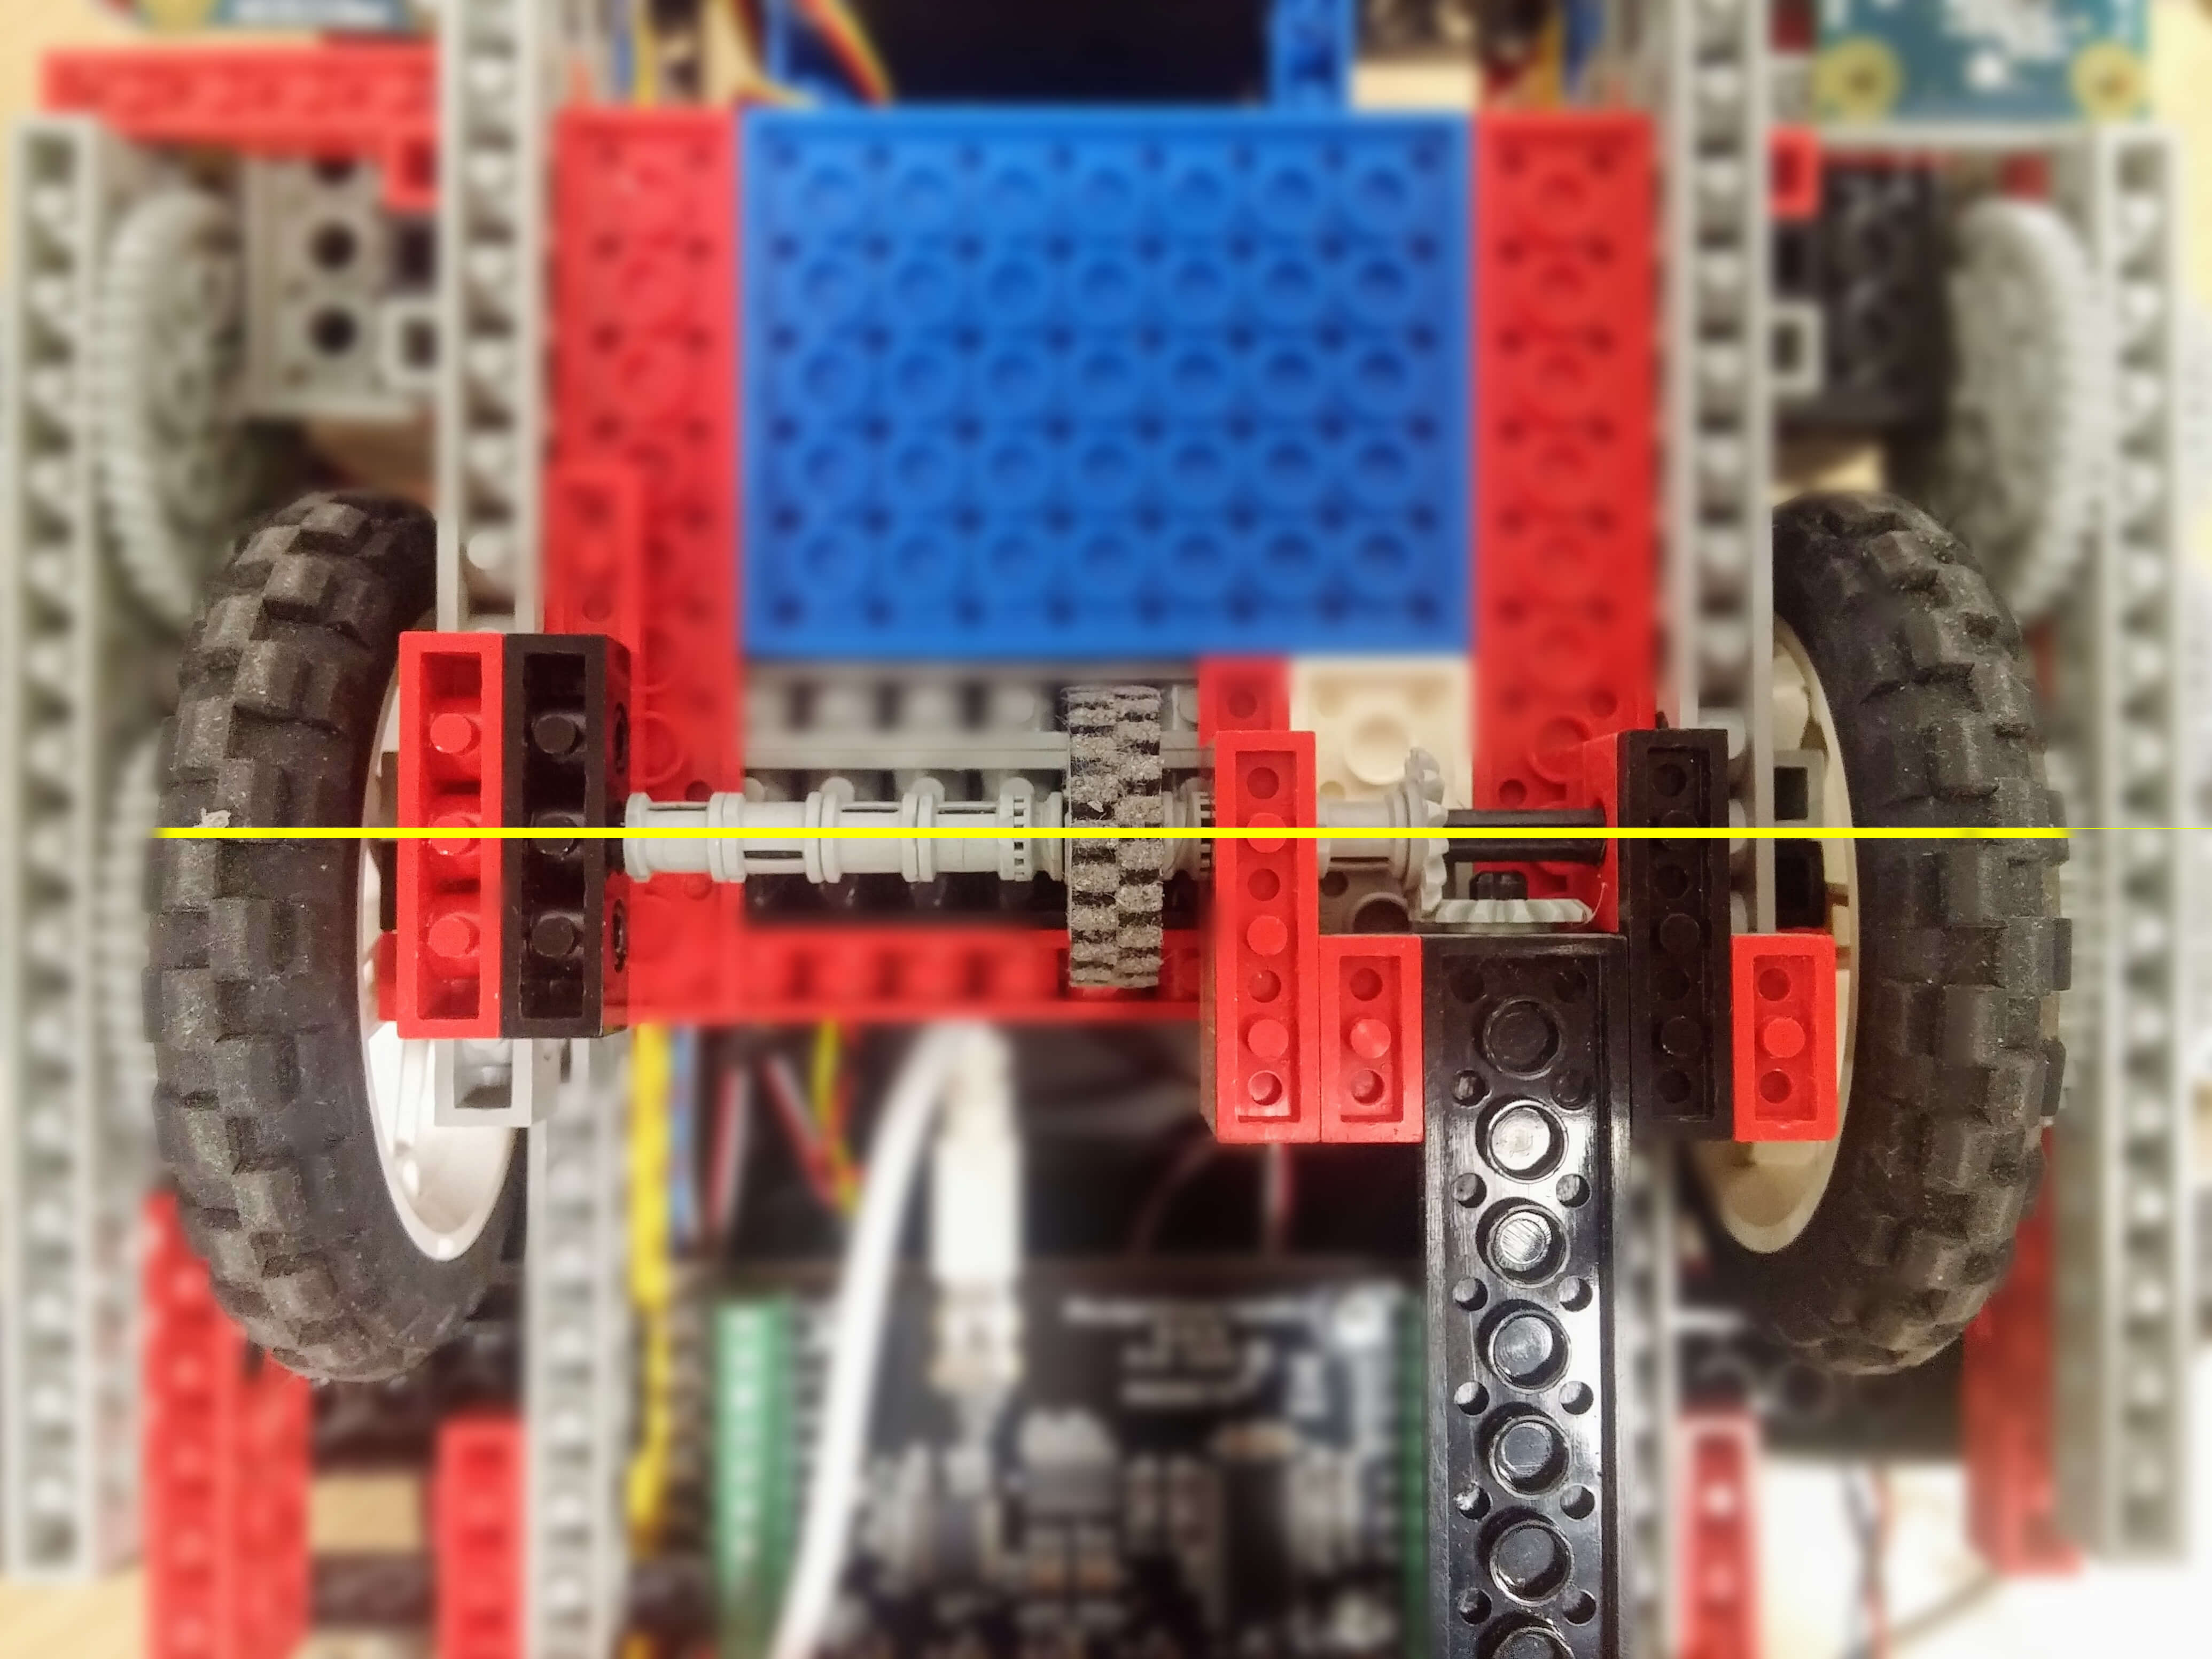
\includegraphics[width=0.7\linewidth]{res/robot-pics/pivot-wheel-layout.jpg}
    \caption{}
    \label{fig:}
\end{figure}

\begin{figure}[ht]
    \centering
    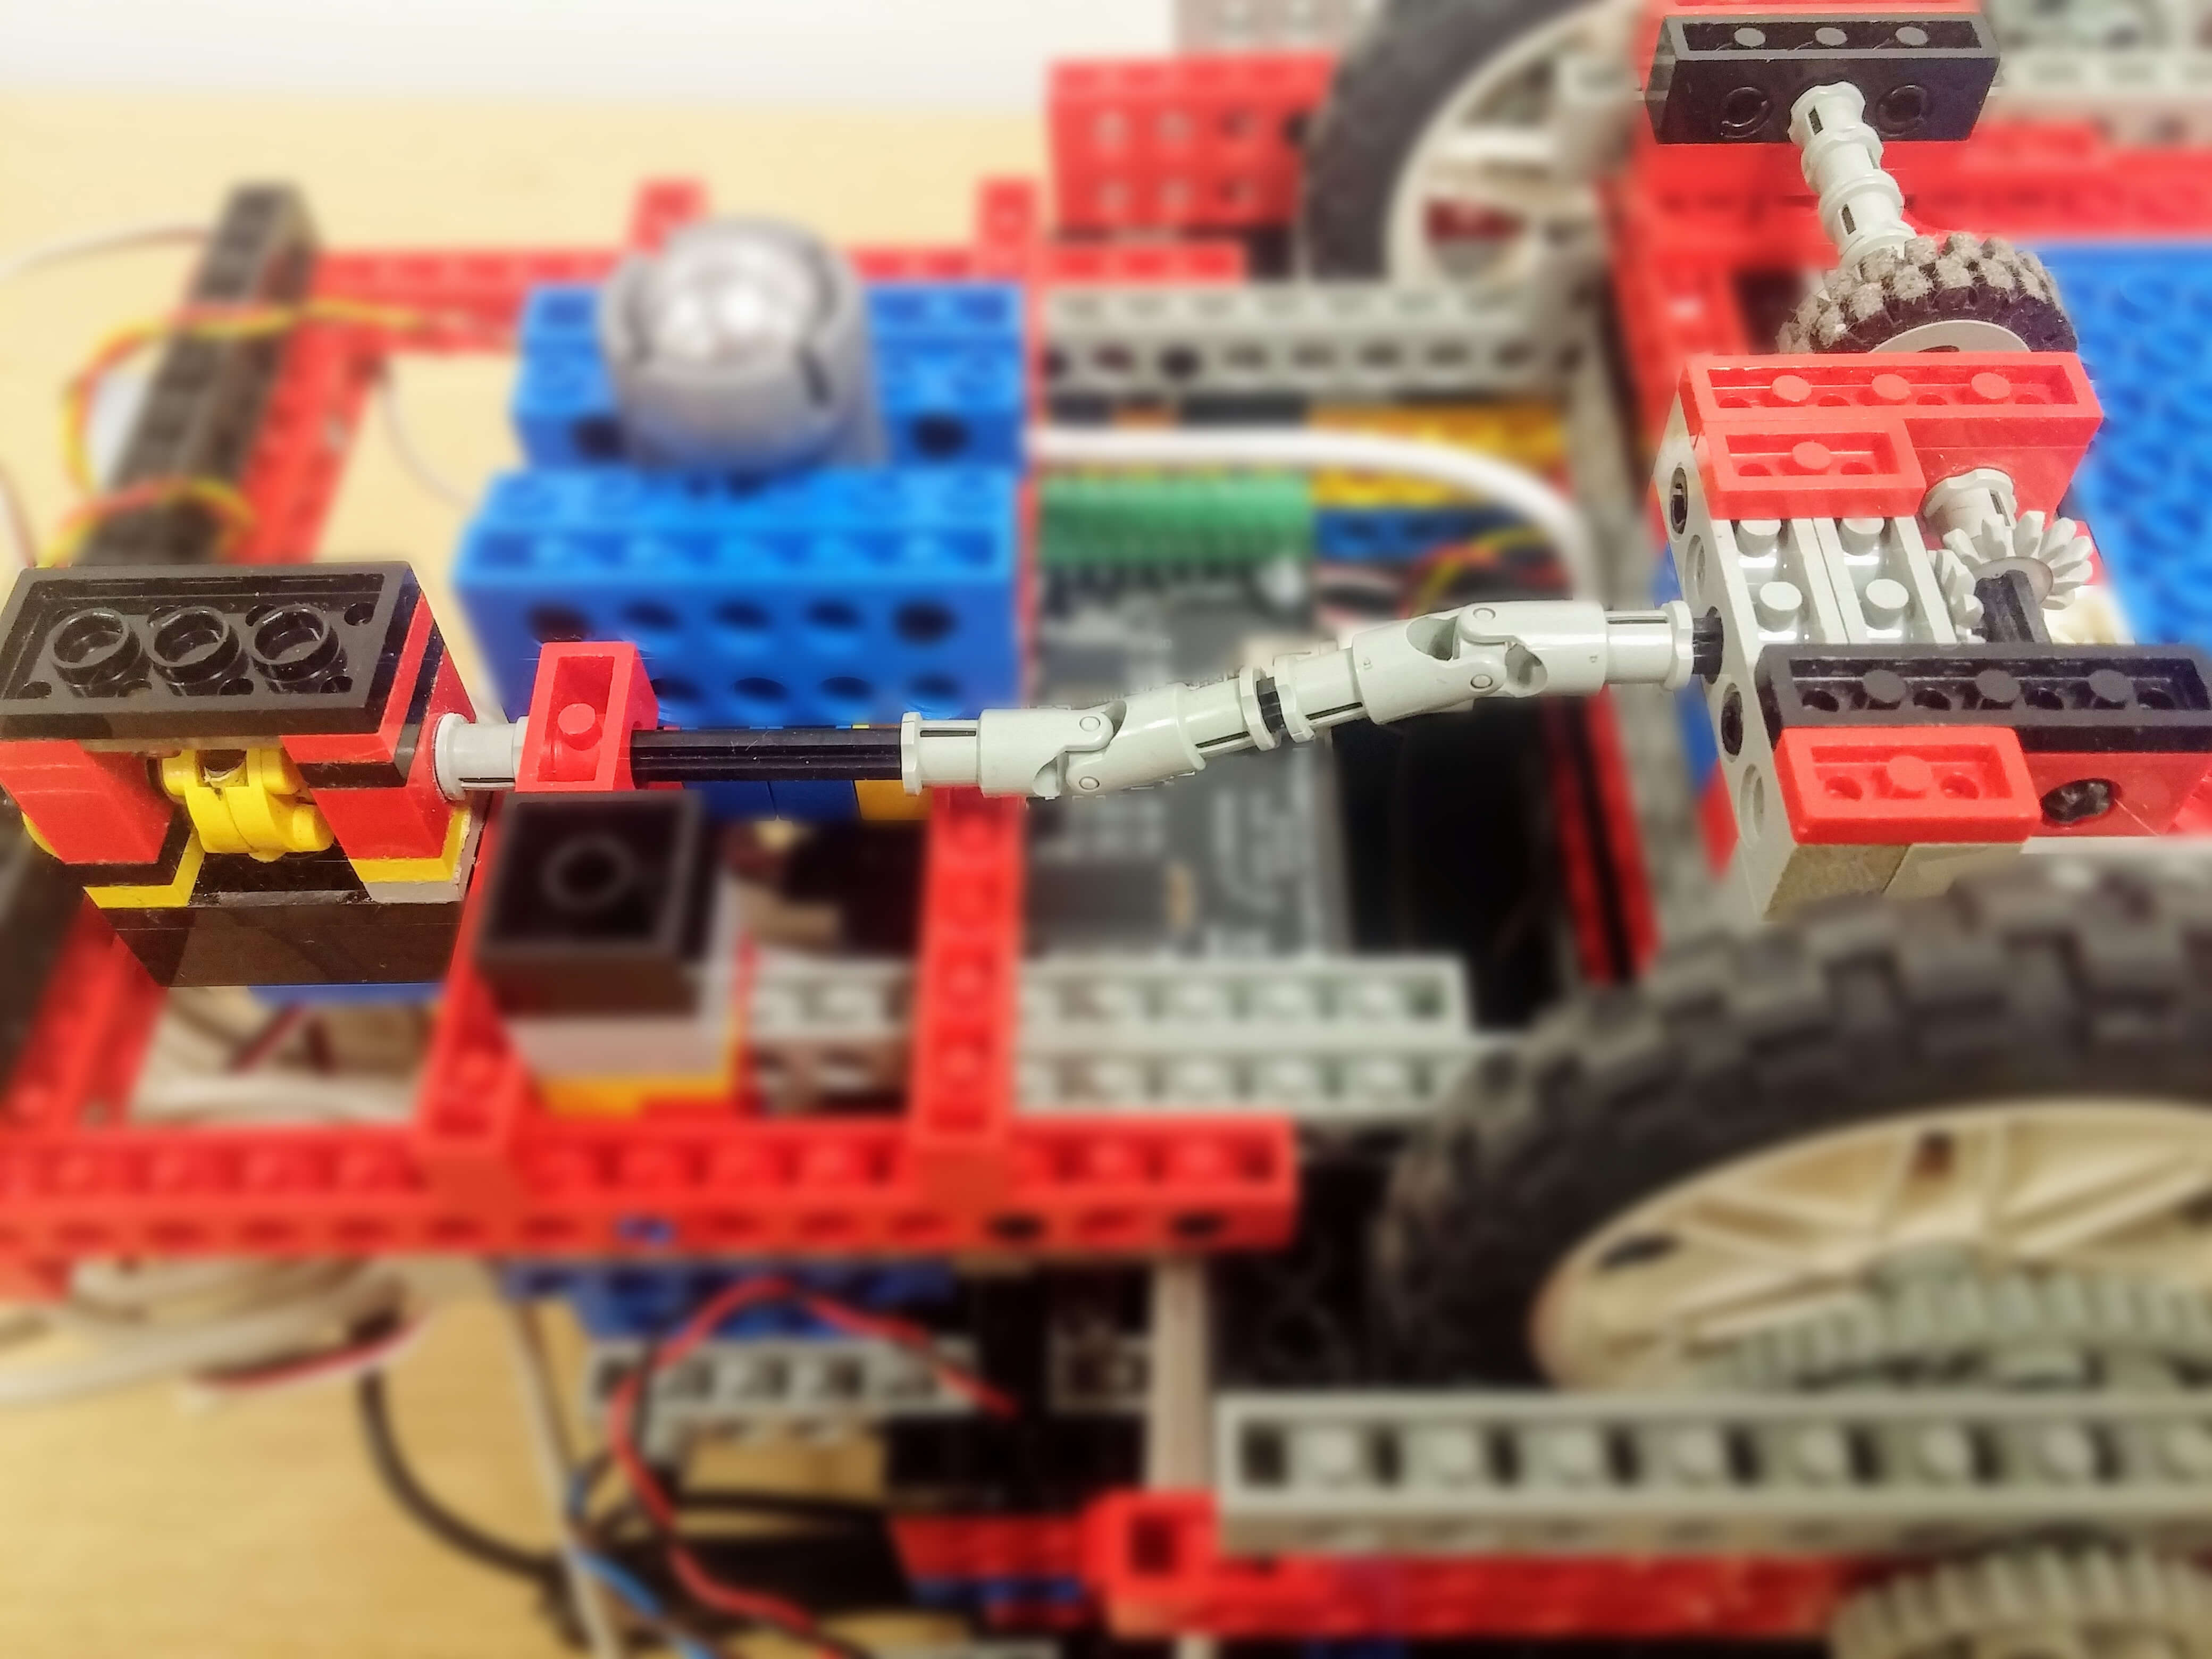
\includegraphics[width=0.7\linewidth]{res/robot-pics/pivot-wheel-sensor.jpg}
    \caption{}
    \label{fig:}
\end{figure}

\begin{figure}[ht]
    \centering
    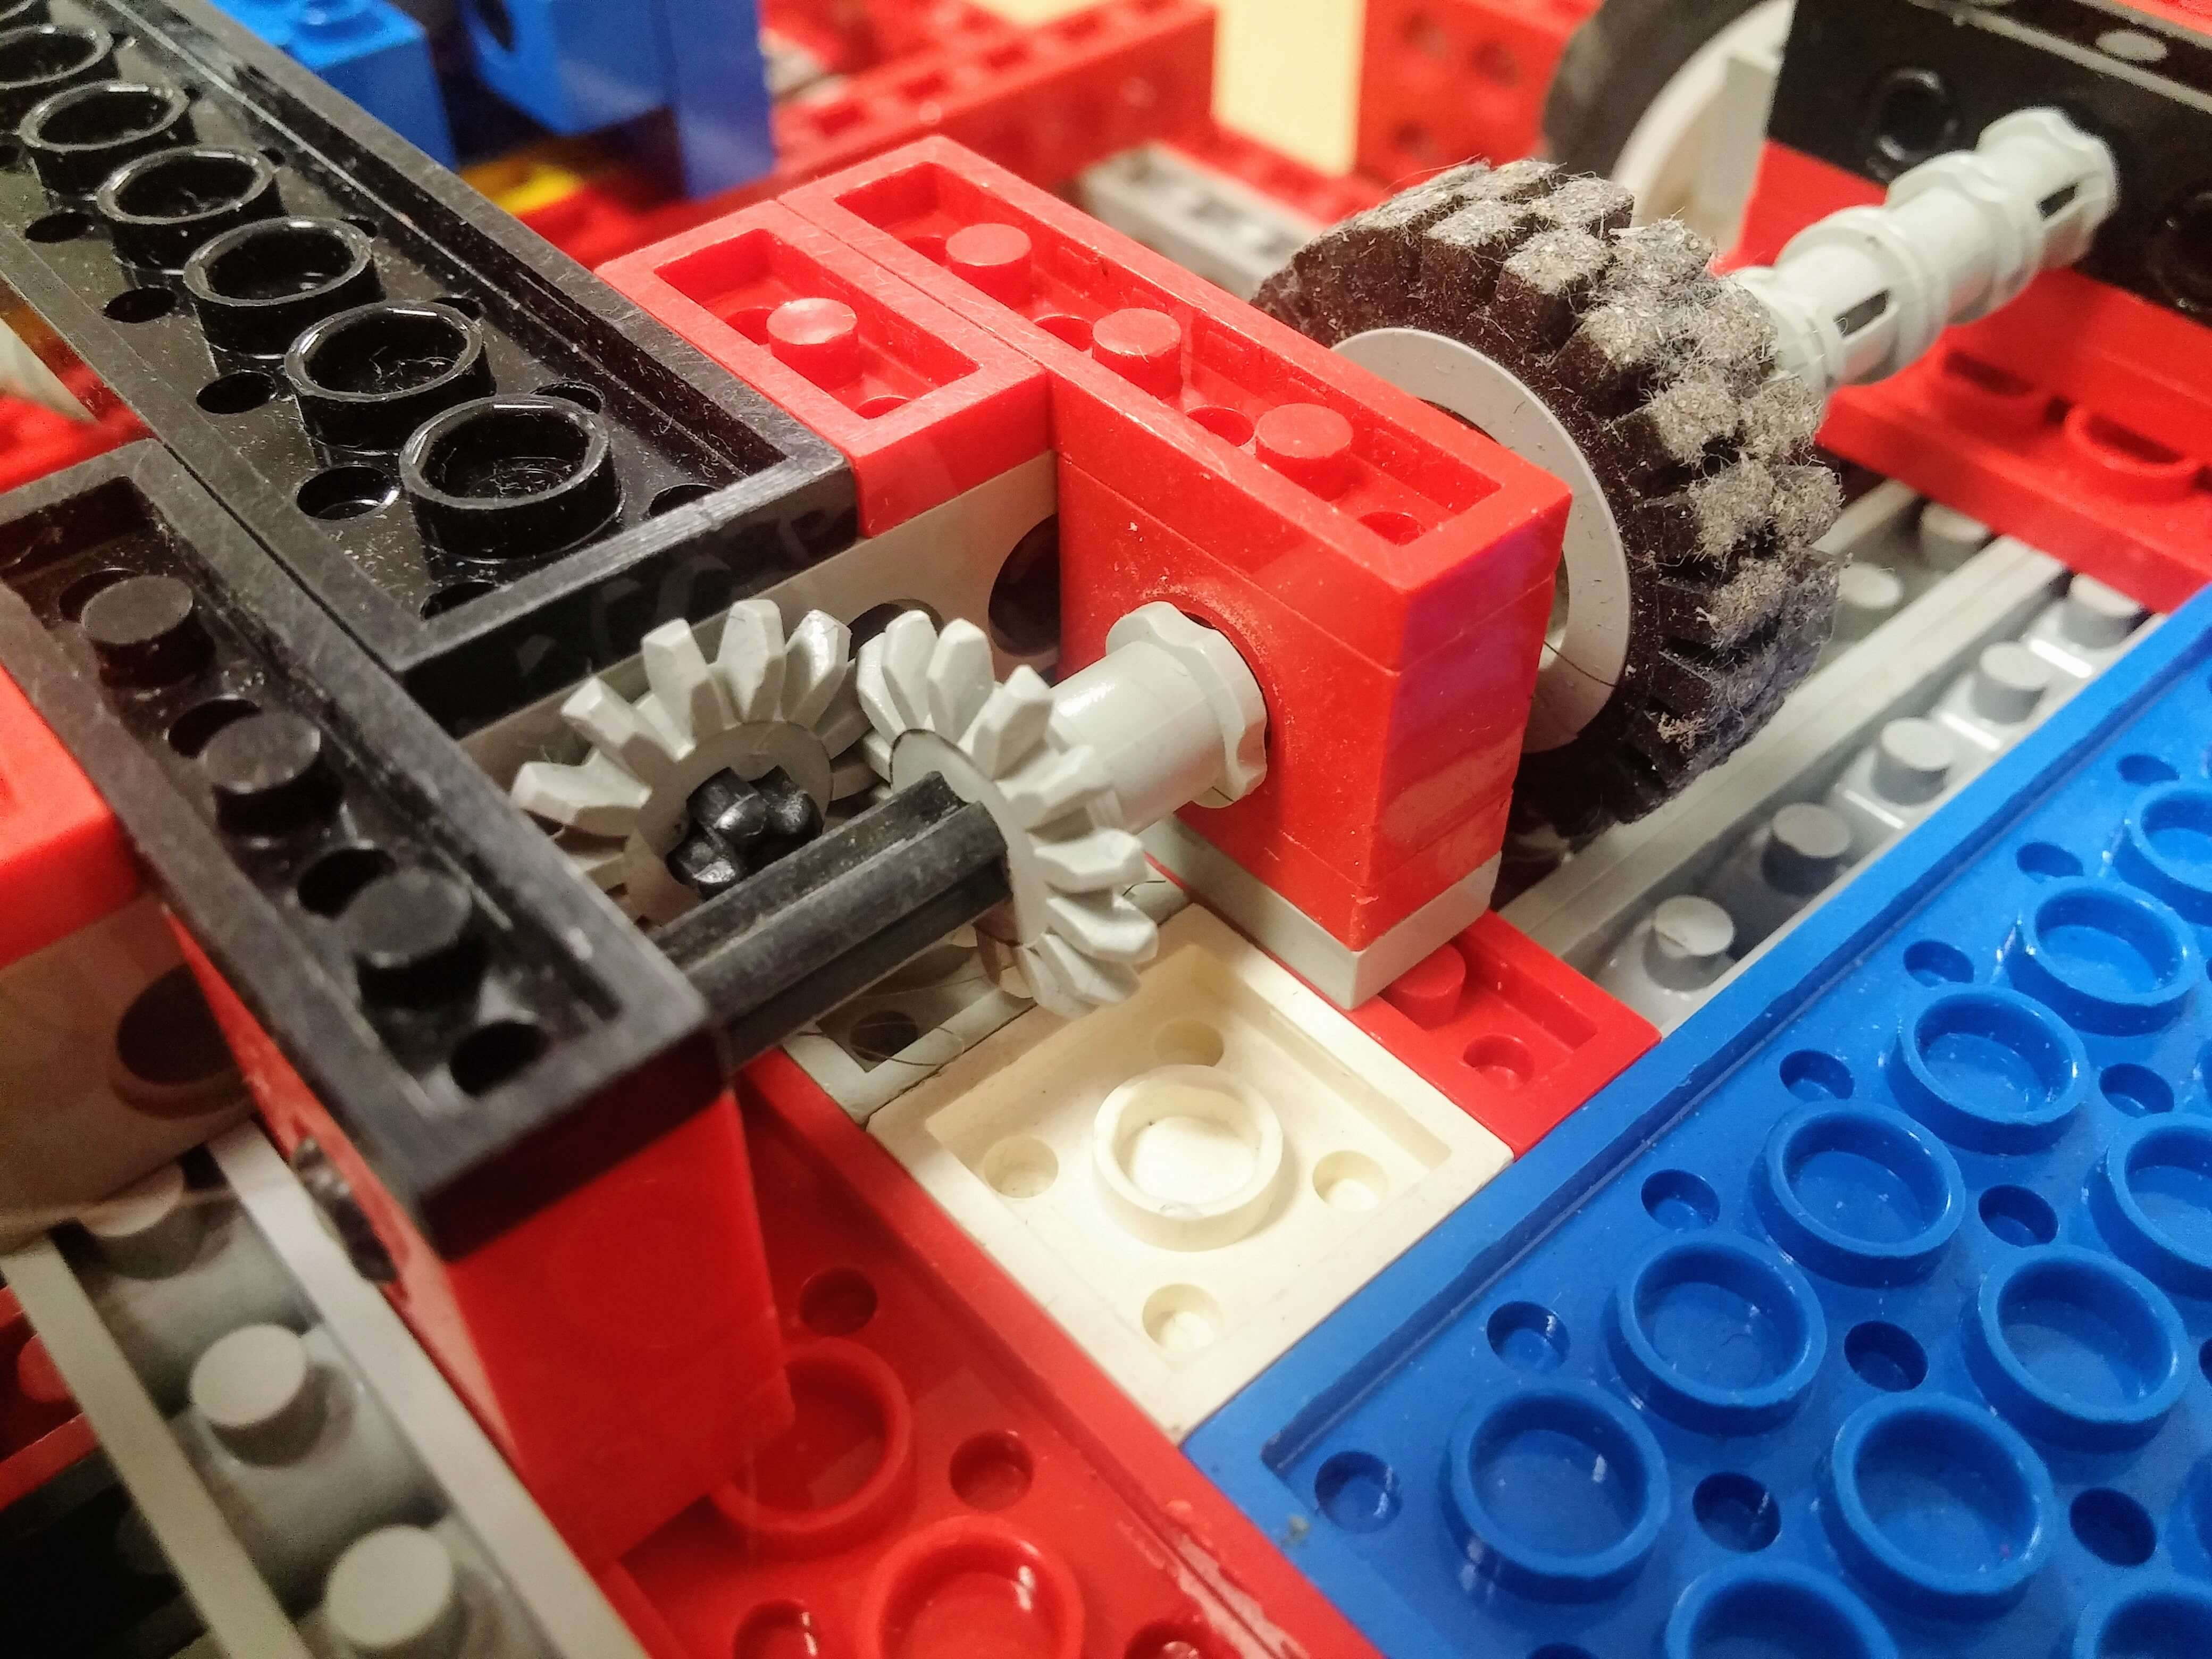
\includegraphics[width=0.7\linewidth]{res/robot-pics/pivot-wheel-axel-transfer.jpg}
    \caption{}
    \label{fig:}
\end{figure}

\subsubsection{Whiskers}
\label{sec:whiskers}

% - - - - - - - - - - - - - - - - - - - - - - - - - - -

For the control program you should provide a flow diagram or pseudo-code description, and again explain the reasoning that led to this solution.

This is likely to be the longest section of the report. Do not include code except for short snippets that help explain a crucial part of the program you created.

Avoid repetition and refer to other peoples' work instead of describing well known algorithms. (1400 words)

\newpage
